\chapter{Real-time $360 ^{\circ} $ cars rendering from multiple images with Gaussian Splatting}
\label{chapter:gausssplat}

\chapterwithfigures{\nameref*{chapter:gausssplat}} 
\chapterwithtables{\nameref*{chapter:gausssplat}}

\ifthenelse{\boolean{skipGauss}}{\endinput}{}

While 3D reconstruction landscape in deep learning has been entirely reshaped over the last few years with the \ac{NeRF} based framework, such technology remain ineffective for any industrial applications, both from a training (expressed in hours or even days) and inference perspective(regarding the milions of network queries required to render an image). \ac{GS} methods recently appeared as a well balanced trade-off between rendering quality and training/inference requirements. Contrary to \ac{NeRF} based methods, \ac{GS} does not rely on any \ac{NN} architecture. We propose through this last chapter a system that stabilised an unbounded scene depicting a single car to perform a stabilized $360 ^{\circ} $ rendering. We highlight in which extend such a learning-based method is better than a full image wrapping pipeline and develop the different modules we plugged in our pipeline to reach the best rendering quality. Our experiments and corresponding ablation studies extensively confirm that such a pipeline is efficient for an industrial application. 

\section{Introduction}
This final chapter extends the latest two ones that were mostly focused toward a research academic perspective. Core motivation rather lies here on the desire to apply \ac{NVS} latest advances on an industrial project, where processed images resolution are at least $10\times$ higher than ShapeNet-SRN \citep{chang2015shapenet,sitzmann2019scene} ones ($\sim$ 1-2K against $128\times128$). \ac{NeRF} have benefited over the latest few years from massive improvements against several directions; training time, camera pose requirements, inference speed, drastic model weight reduction \textit{etc}. 
However, \ac{NeRF}-based methods suffers from an intrinsic computational bottleneck at inference time. It requires roughly 500 millions \ac{NeRF} queries to generate a squared $2K\times2K$ image. As a direct consequence, one of the most acknowledged state-of-the-art method, termed Mip-NeRF360 \citep{barron2022mip}, is only able to render at < 0.1 \ac{FPS} a 1K resolution image. It would therefore be necessary to deploy a lot of \ac{GPU} resources and engineering refactorization to properly parallelize the source code in order to synthesize novel views at acceptable speed. 

We thus work in this last chapter with a different set of constraints. First concerns the generalizable property we kept in the two previous chapters. We do not aim anymore to build or rely on an algorithm that can synthesize a viewpoint from any image belonging to a specific class. We thus rather want to leverage on \textit{per-scene} framework, that would require a novel training as soon as we work with a new scenario. Furthermore and as mentioned earlier, images we are now working with are closer to what clients could sent to any \ac{AI}-vision SaS company, both regarding resolution and content. Finally, camera poses are no longer available as a ground truth since images Meero has to deal with are unposed. They thus must be first estimated using \ac{SfM} techniques.

Core idea is rather to leverage on the latest advances in neural rendering, mostly on 3D\ac{GS} ones. Contrary to \ac{NeRF}-based methods, that are therefore often too slow to render high-resolution images, 3D\ac{GS} shows an impressive 100 \ac{FPS} performance, withtout relying on any neural network architecture. As soon as 3D\ac{GS} reconstructs the whole 3D scene through a set of 3D colored gaussians, rendering a novel view at a specific viewpoint now only require a camera pose information.

%%%%%%%%%%%%%
%%%%%%%%%%%%
We present on the Figure \ref{fig:gs-vs-homography-view3} how one of the view from the original image set as been stabilized by solely leveraging on image perspective wrapping (center image in Figure \ref{fig:gs-vs-homography-view3}). The same rendered view from the learned \ac{GS} scene is depicted on the right side of Figure \ref{fig:gs-vs-homography-view3}. As the entire 3D scene structure has been learned and is explicitly stored as a gaussian point cloud, one can render it at any locations and synthesise the whole car. The rendering comes from the vanilla \ac{GS} framework, without any of our modifications.

\begin{figure*}[htb!]
  \center
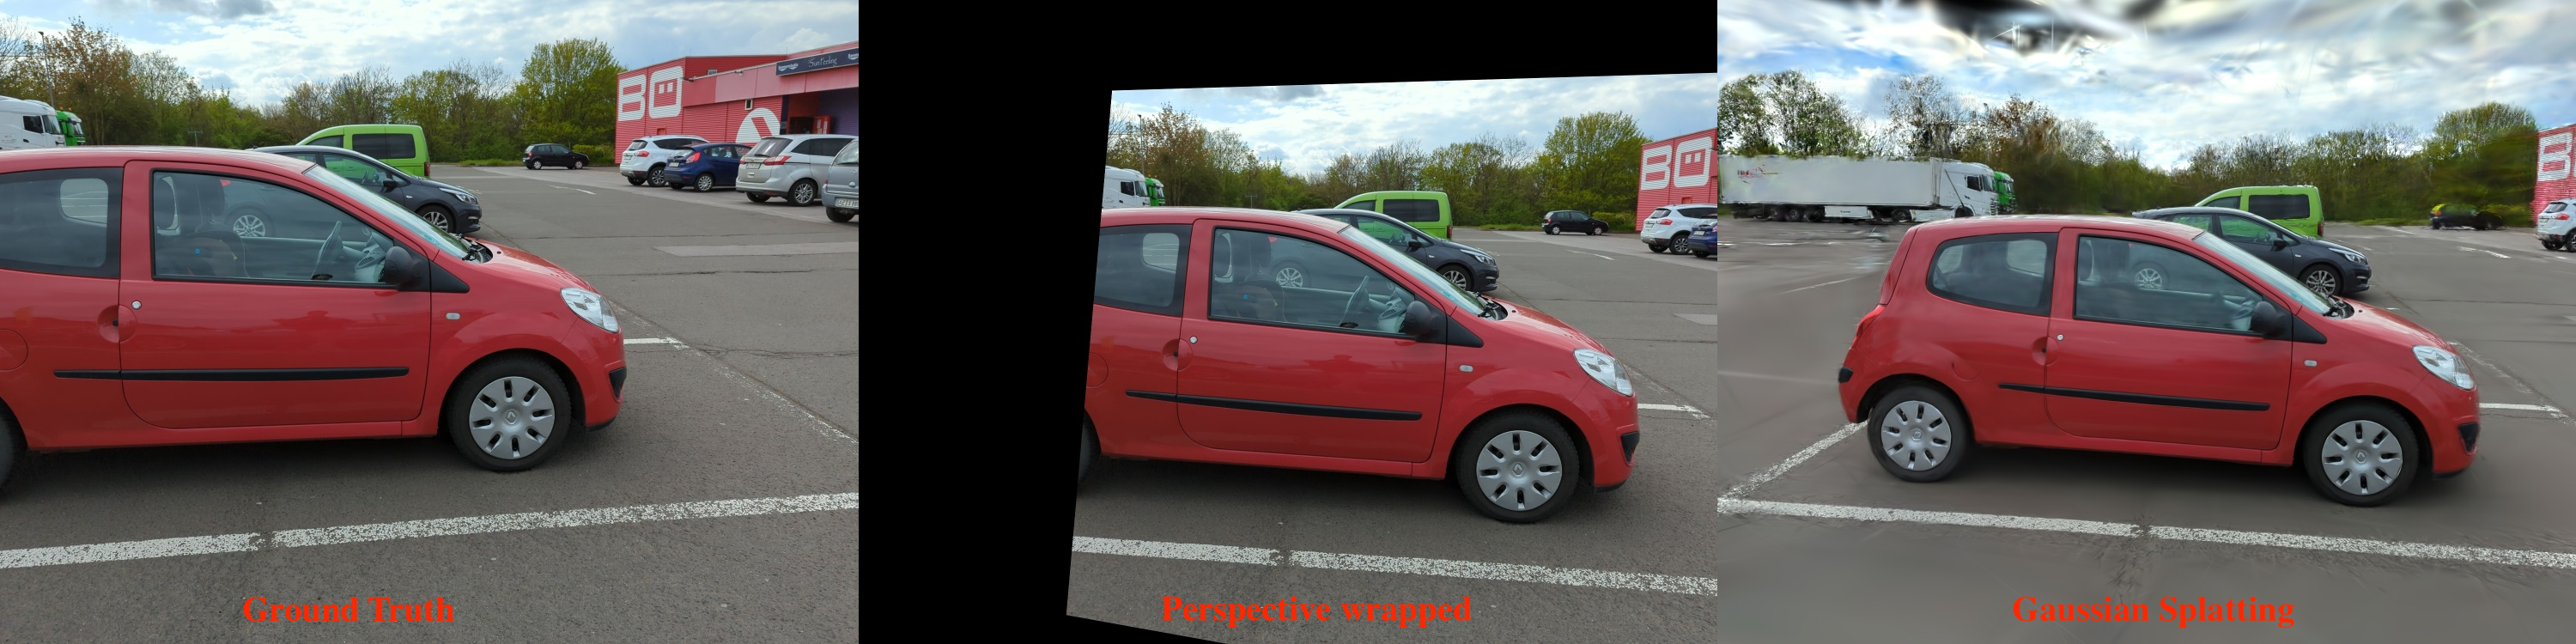
\includegraphics[width=\linewidth]{images/gaussiansplatting/perspective-vs-gs.png}
\caption{\textbf{Perspective transformation and Gaussian Splatting based stabilisation. } Contrary to the homography-based solution, trained GS scene is able to render the whole car. Whereas the car is now properly centred on the view, the perspective-wrapped car is incomplete as the corresponding transformation to apply was too drastic.}
\label{fig:gs-vs-homography-view3}
\end{figure*}

Applying such a transformation to the entire scene, frame by frame, would allow to stabilized the scene entirely. However, as soon as a source view cannot depict the whole car, such an image-based method will fail. 

 
\begin{table}[h!]
  \centering
   \caption{\textbf{Properties of interest benchmark for $360^{\circ}$ scene stabilization.}}
  \begin{tabular}{lcccc}
  \hline
  
    & Complex Reflections & Occlusions & Rendering time & \\
  \hline
  \hline
  Image warp.  & \xmark & \xmark & \cmark \\
  NeRF & \cmark & \cmark & \xmark\\
  GS  & \xmark & \cmark & \cmark \\
  Ours  & \cmark & \cmark & \cmark \\
  \hline
  \label{tab:gs-comp}
  \end{tabular}
\end{table}

We thus leverage  on 3D\ac{GS}-based techniques \citep{kerbl20233d} to build up a $360^{\circ}$ spin stabilisation pipeline for unbounded scenes. As soon as such a 3D reconstruction system primarily aims to live in a production pipeline for an industrial application, presented methods and experiments extensively focused onto a single scene, that could be one from a Meero car dealership client. As presented in Table \ref{tab:gs-comp}, the pipeline we designed on top of the 3D\ac{GS} one allow us to also tackle reflection and transparent surfaces, without hurting training time or inference performances. 

In summary, we build up an improved 3D reconstruction pipeline based on a vanilla 3D\ac{GS} architecture that allows to synthetically render a learn 3D scene at novel viewpoints. Our contributions in this section are three-fold: 
\begin{itemize}
  \item We extend the original sparse \ac{SfM} point cloud from COLMAP. A 3D visual hull is computed to sample as many points as required to complete the point cloud. 
  \item We direclty leverages upon \citep{malarz2023gaussian} work to make gaussian's opacity view-dependent. Such a modification allows us to better render transparents and reflective surfaces. 
  \item We integrate into our architecture a corrected Adaptative Density Control strategy \citep{zhang2024pixelgs}. 
    
\end{itemize}

\section{Background: Gaussian Splatting}
We present below a first complete overview of the underlying concepts behind 3D\ac{GS} \citep{kerbl20233d}. It leverages on 3D Gaussian primitives to explicitly model the 3D scene and a fully differentiable pipeline that can solely be supervised at 2D-image level. 

\subsection{Initialization} From a sparse coloured \ac{SfM}-3D point cloud obtained with COLMAP and referred as $\mathcal{P}\in\mathbb{R}^{N\times(3+3)}$, an associated set of 3D Gaussians $\{\mathcal{G}_{k}|k=1,...,K\}$ is built. Each primitive $\mathcal{G}_{k}$ has therefore an attached set of learnable attributes, defined in Table \ref{tab:gauss-param}, and expressed in the world coordinate system.

\begin{table}[h!]
  \centering
   \caption{Per gaussian $\mathcal{G}_{k} $  parameters that need to be optimized.}
  \begin{tabular}{lcc}
  \hline
  Parameter  & Size & Note \\
  \hline
  Position (mean)  $\mu^{(k)}_{3D}$ & 3 & 3D vector  \\
  3D Covariance $\Sigma^{(k)}_{3D}$ & 7 & 4D vector + 3D vector \\
  Opacity  $o^{(k)}$ & 1 & scalar \\
  SH coefficients  $c^{(k)}$ & 48 & 4 bands of \ac{SH}; $(1+3+5+7)\times3$ \\
  \hline
  Total (per Gaussian)  & 59 & \\
  \hline
  \end{tabular}
 
  \label{tab:gauss-param}
\end{table}

While mean, color and opacity can be optimised without any constraints with \ac{SGD} algorithm, $\Sigma^{(k)}_{3D}$ has to remain semi-definite positive \footnote{\textit{i.e} $ \forall a \in \mathbb{R}^{3}: a^{T}\Sigma^{(k)}_{3D}a \geq 0$} during training to represent a meaningful 3D coviance matrix. As holding this constraint during the optimization would be impossible, $\Sigma^{(k)}_{3D}$ is factorized (as an eigendecomposition) in the world coordinate system via with a rotation matrix $O_{k}$ (analytically expressed as a four-dimentional quaternion $q_{k}$) and a scaling 3D vector $s_{k}$: 

\begin{equation}
    \Sigma^{(k)}_{3D} = O_{k}s_{k}s_{k}^{T}O_{k}^{T}
\end{equation}

Since any matrix expressed as $A^{T}A$ is always semi-definite positive, $\Sigma^{(k)}_{3D}$ is now properly constrained. 

Considering any point \textit{p} in the world 3D space, the geometry of a primitive $\mathcal{G}_{k}$ has an influence over \textit{p} that can be expressed through: 

\begin{equation}
  \mathcal{G}_{k}(p) = \exp \left(-\frac{1}{2}(p-\mu^{(k)}_{3D})^{T}(\Sigma^{(k)}_{3D})^{-1}(p-\mu^{(k)}_{3D})\right)
\end{equation}

\subsection{3D Gaussian projection} The 3D Gaussian parameters are optimised during training by only leveraging on an image-based supervision signal. The 3D ellipsoids must thus be render on 2D image plane in a differentiable manner and a corresponding 2D mean and covariance need to be derived from $\mu^{(k)}_{3D}$ and $\Sigma^{(k)}_{3D}$ for each primitive using EWA splatting \citep{zwicker2001ewa}. 

We breakdown the different steps required to obtain those rendered 3D gaussians onto 2D image plane. 

Given any viewpoint we want to render, any 3D primitive $\mathcal{G}_{k}$ expressed in world coordinate has to be expressed in camera coordinate system first. Let's denote corresponding world-to-camera extrinsic matrix $W=[R|t]$. 

The 3D mean of $\mathcal{G}_{k}$, denoted $\mu^{(k)}_{cc}$, is easly expressed through: 

\begin{equation}
  \mu^{(k)}_{cc} = R\times \mu^{(k)}_{3D}+t
\end{equation}

while the covariance $\Sigma^{(k)}_{3D}$ can be obtained trough: 

\begin{equation}
  \Sigma^{(k)}_{cc}= R\Sigma^{(k)}_{3D}R^{T}
  \label{eq:gs-3dcov-transfrom}
\end{equation}

The whole developement of such an expression for $\Sigma^{(k)}_{cc}$ is given in Appendix \ref{appendix:cov}. 

As soon as the volume rendering needs to be performed in the ray space \footnote{Computation is easier in this space since viewing rays are parallel to a coordinate axis}, which is a non-cartesian coordinate system, original 3D\ac{GS} project the primitive $\mathcal{G}_{k}$ (expressed in the camera space) onto the $z=1$ plane through the projective transform $\phi$: 

\begin{equation}
  \phi(p') = [p_{x}'/p_{z}',p_{y}'/p_{z}',1] = p'\times(p_{0}^{T}p')^{-1}
\end{equation}
where $p'=Wp = [p_{x}',p_{y}',p_{z}']^{T}$ is a 3D point expressed in camera coordinate system and and $p_{0} = [0, 0, 1]^{T}$. \newline

However, such a projective function $\phi$ is not affine (as it was the case for $W$ during the world to camera space transform) and one need to locally approximate $\phi$ (for each primitive) with an affine transformation using Taylor first order series: 

\begin{equation}
  \label{eq:affine_transform}
  \phi(p') = \approx \phi(\mu_{cc}) + \frac{\partial \phi}{\partial p'}(\mu_{cc})(p' - \mu_{cc})
\end{equation}

whereas we denote $J = \frac{\partial \phi}{\partial p'}(\mu_{cc})$ as the jacobian of the affine approximation of $\phi$. 

One can derive from $J$ and $\phi$ an expression for $\mu^{(k)}_{2D}$ and $\Sigma^{(k)}_{2D}$, the 2D projected gaussian primitive, termed  $g_{k}$, in the image space. Complete derivation is available in Appendix \ref{appendix:cov} and we thus end with: 

\begin{equation}
  g_{k}(x) = \exp(-\frac{1}{2}(x-\mu^{(k)}_{2D})^{T}(\Sigma^{(k)}_{2D})^{-1}(p-\mu^{(k)}_{2D}))
\end{equation}

3D\ac{GS} seminal work \citep{kerbl20233d} finally performs alpha blending to derive the color $\hat{c}(x)$ of the pixel: 

\begin{equation}
\label{eq:gs-alpha-blending}
  \hat{c}(x) = \sum_{k=1}^{K}c^{(k)}\alpha^{(k)}\prod_{j=1}^{k-1}(1-\alpha^{(j)})
\end{equation}

\begin{equation}
\label{eq:gs-alpha-def}
  \alpha^{(k)} = o^{(k)}g_{k}(x)
\end{equation}

where primitive’s depth order are sorted from 1 to K. \newline

\subsection{Adaptative Density Control strategy} 
As the original \ac{SfM} point cloud can be extremely sparse, authors from \citep{kerbl20233d} implement both a densification and pruning strategy during training, termed \ac{ADC}. 

The pruning is quite simple yet effective: any 3D gaussian $\mathcal{G}_{k}$ that has an opacity $o^{(k)}$ below a fixed threshold $\epsilon_{o}$ during training is removed from the gaussian set. 

The densification strategy requires to both address under-reconstructed areas (where an insufficient number of gaussians are presents) and over-reconstructed areas (where gaussians are too large) of the scene. Small gaussians are thus cloned in those under-reconstructed areas whereas large ones are splited into two new gaussians by leveraging on view-space positional gradients, expressed for each gaussian primitive $\mathcal{G}_{k}$ as : 

\begin{equation}
   \nabla_{\mu_{k}}L= ||\frac{\partial L_{\pi}}{\partial \mu_{k}^{\pi}}|| = \sqrt{\left(\frac{\partial L_{\pi}}{\partial \mu_{ndc,x}^{k,\pi}}\right)^{2} + \left(\frac{\partial L_{\pi}}{\partial \mu_{ndc,y}^{k,\pi}}\right)^{2}}
\end{equation}

where $L_{\pi}$ denotes the loss under viewpoint $\pi$. Such a gradient magnitude is tracked and averaged over all the rendered views $\pi \in \Pi$ during 100 iterations. As soon as: 

\begin{equation}
\frac{\sum \limits_{\pi \in \Pi} ||\frac{\partial L_{\pi}}{\partial \mu_{k}^{\pi}}||}{\sum \limits_{\pi \in \Pi} 1} > \tau_{pos}
\label{eq:adc-original}
\end{equation}

holds for gaussian primitive $\mathcal{G}_{k}$, the latter is either splited or cloned depending on its size. Largest eigenvalue of $\Sigma_{k}$ is used to status on $\mathcal{G}_{k}$ size: if such an eigenvalue is above another fixed user defined threshold, primitive is splited, cloned otherwise. \newline

\subsection{Training} 
Gaussians parameters are learned during training through the vanilla \ac{SGD} optimization procedure. The corresponding loss function is expressed through: 
\begin{equation}
    \mathcal{L} = (1-\lambda)\mathcal{L}_{1}(I_{GT},\hat{I}) + \lambda \mathcal{L}_{D-SSIM}(I_{GT},\hat{I})
\end{equation}

\section{Our 3D GS-based pipeline}
We now extensively present in this section the 3D\ac{GS} system we designed for our $360^{\circ}$ spin rendering stabilization problem. We build up our system on top of three distinct strategies, that all consistently improve the overall pipeline. Figure \ref{fig:gs-overview} gives few insights regarding how such a pipeline is built. \newline

\begin{figure*}[htb!]
    \center
  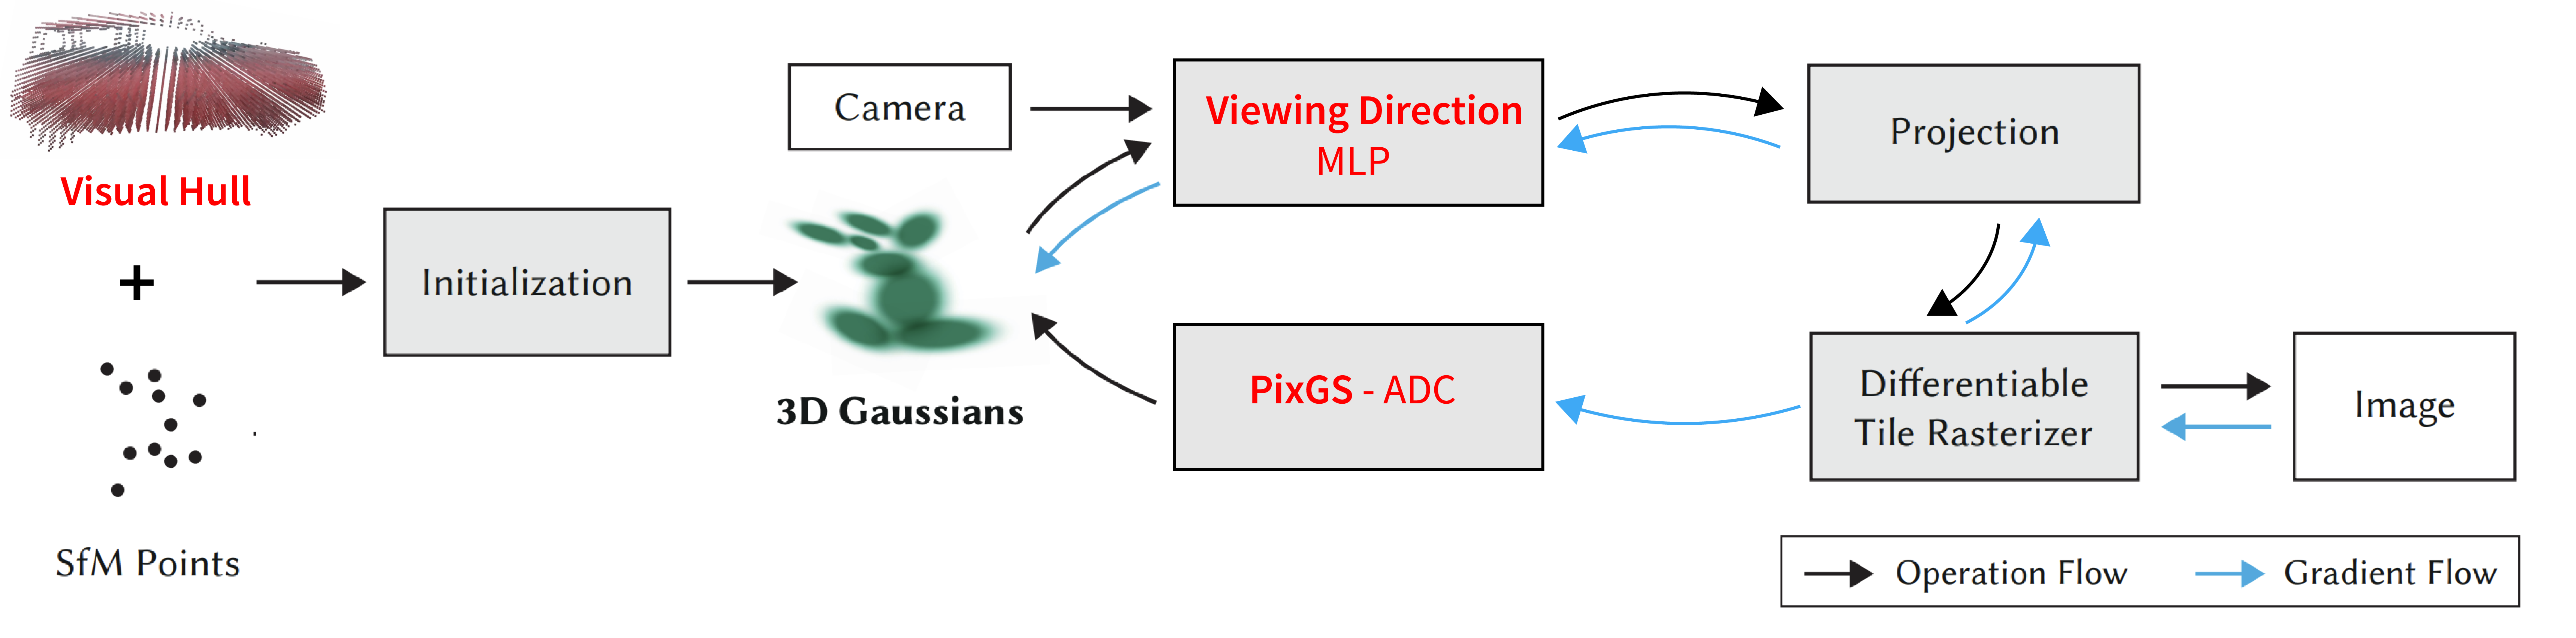
\includegraphics[width=\linewidth]{images/gaussiansplatting/overview_pipeline.png}
  \caption{\textbf{Gaussian Splatting pipeline overview.} Starting from a sparse 3D point cloud, GS is designed on a lightweight and differentiable pipeline that does not involve any deep or shallow neural architectures. \textit{Original illustration comes from the seminal paper}\citep{kerbl20233d} while our modifications are highlighted in \textcolor{red}{red}.}
  \label{fig:gs-overview}
\end{figure*}

\subsection{Visual Hull}

We present in this first section a complementary way to get another initial point cloud $\mathcal{P}$ to start GS scene training. 

\begin{figure*}[htbp!]
    \center
  \includegraphics[width=\linewidth]{images/gaussiansplatting/image_sift.png}
  \caption{\textbf{SIFT correspondence between 2 closed views} SIFT keypoints detection and matching from COLMAP struggle a lot on such a reflective scene. Only a very limited number of key-points has been properly matched (in bold).}
  \label{fig:sift-colmap}
\end{figure*}

As cars surface are extremely prone to light reflections, most of the 3D points produced by the COLMAP algorithm do not lie on the car. Indeed, perform SIFT keypoints detection and matching in 2D in those regions is a challenging task and corresponding results can be seen on Figure \ref{fig:sift-colmap}. Only a very limited number of SIFT points have been properly matched each other on these two views. Such a poor detection and matching performance led to a 
final point cloud that is extremely sparse: $\mathcal{P}$ is only made of a few thousands points and most of them do not live on the car surface, as seen on Figure \ref{fig:sfm-colmap-pc}. 

\begin{figure*}[htbp!]
    \center
  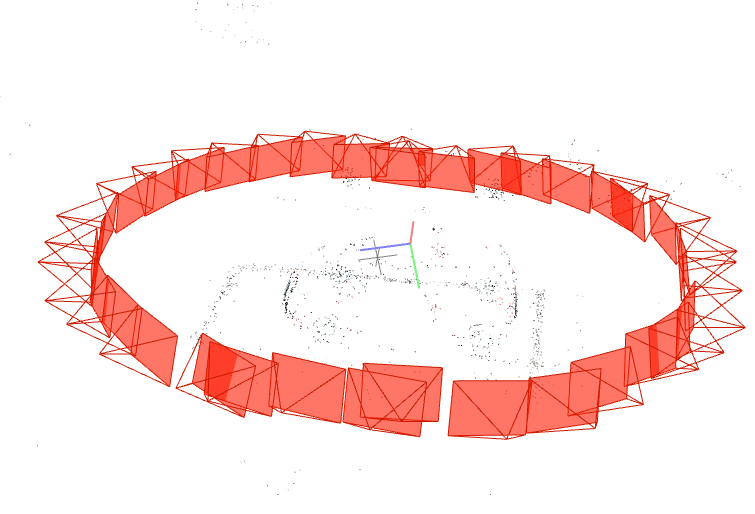
\includegraphics[width=.8\linewidth]{images/gaussiansplatting/colmap_sparsePC.png}
  \caption{\textbf{Final SfM point cloud with predicted camera poses} Wheareas 36 views were involved in the \ac{SfM}-point cloud construction, only few points lie on the car surface we aim to reconstruct in 3D.}
  \label{fig:sfm-colmap-pc}
\end{figure*}

\begin{figure}[htpb!]
  \centering
  \begin{subfigure}[b]{0.48\linewidth}
    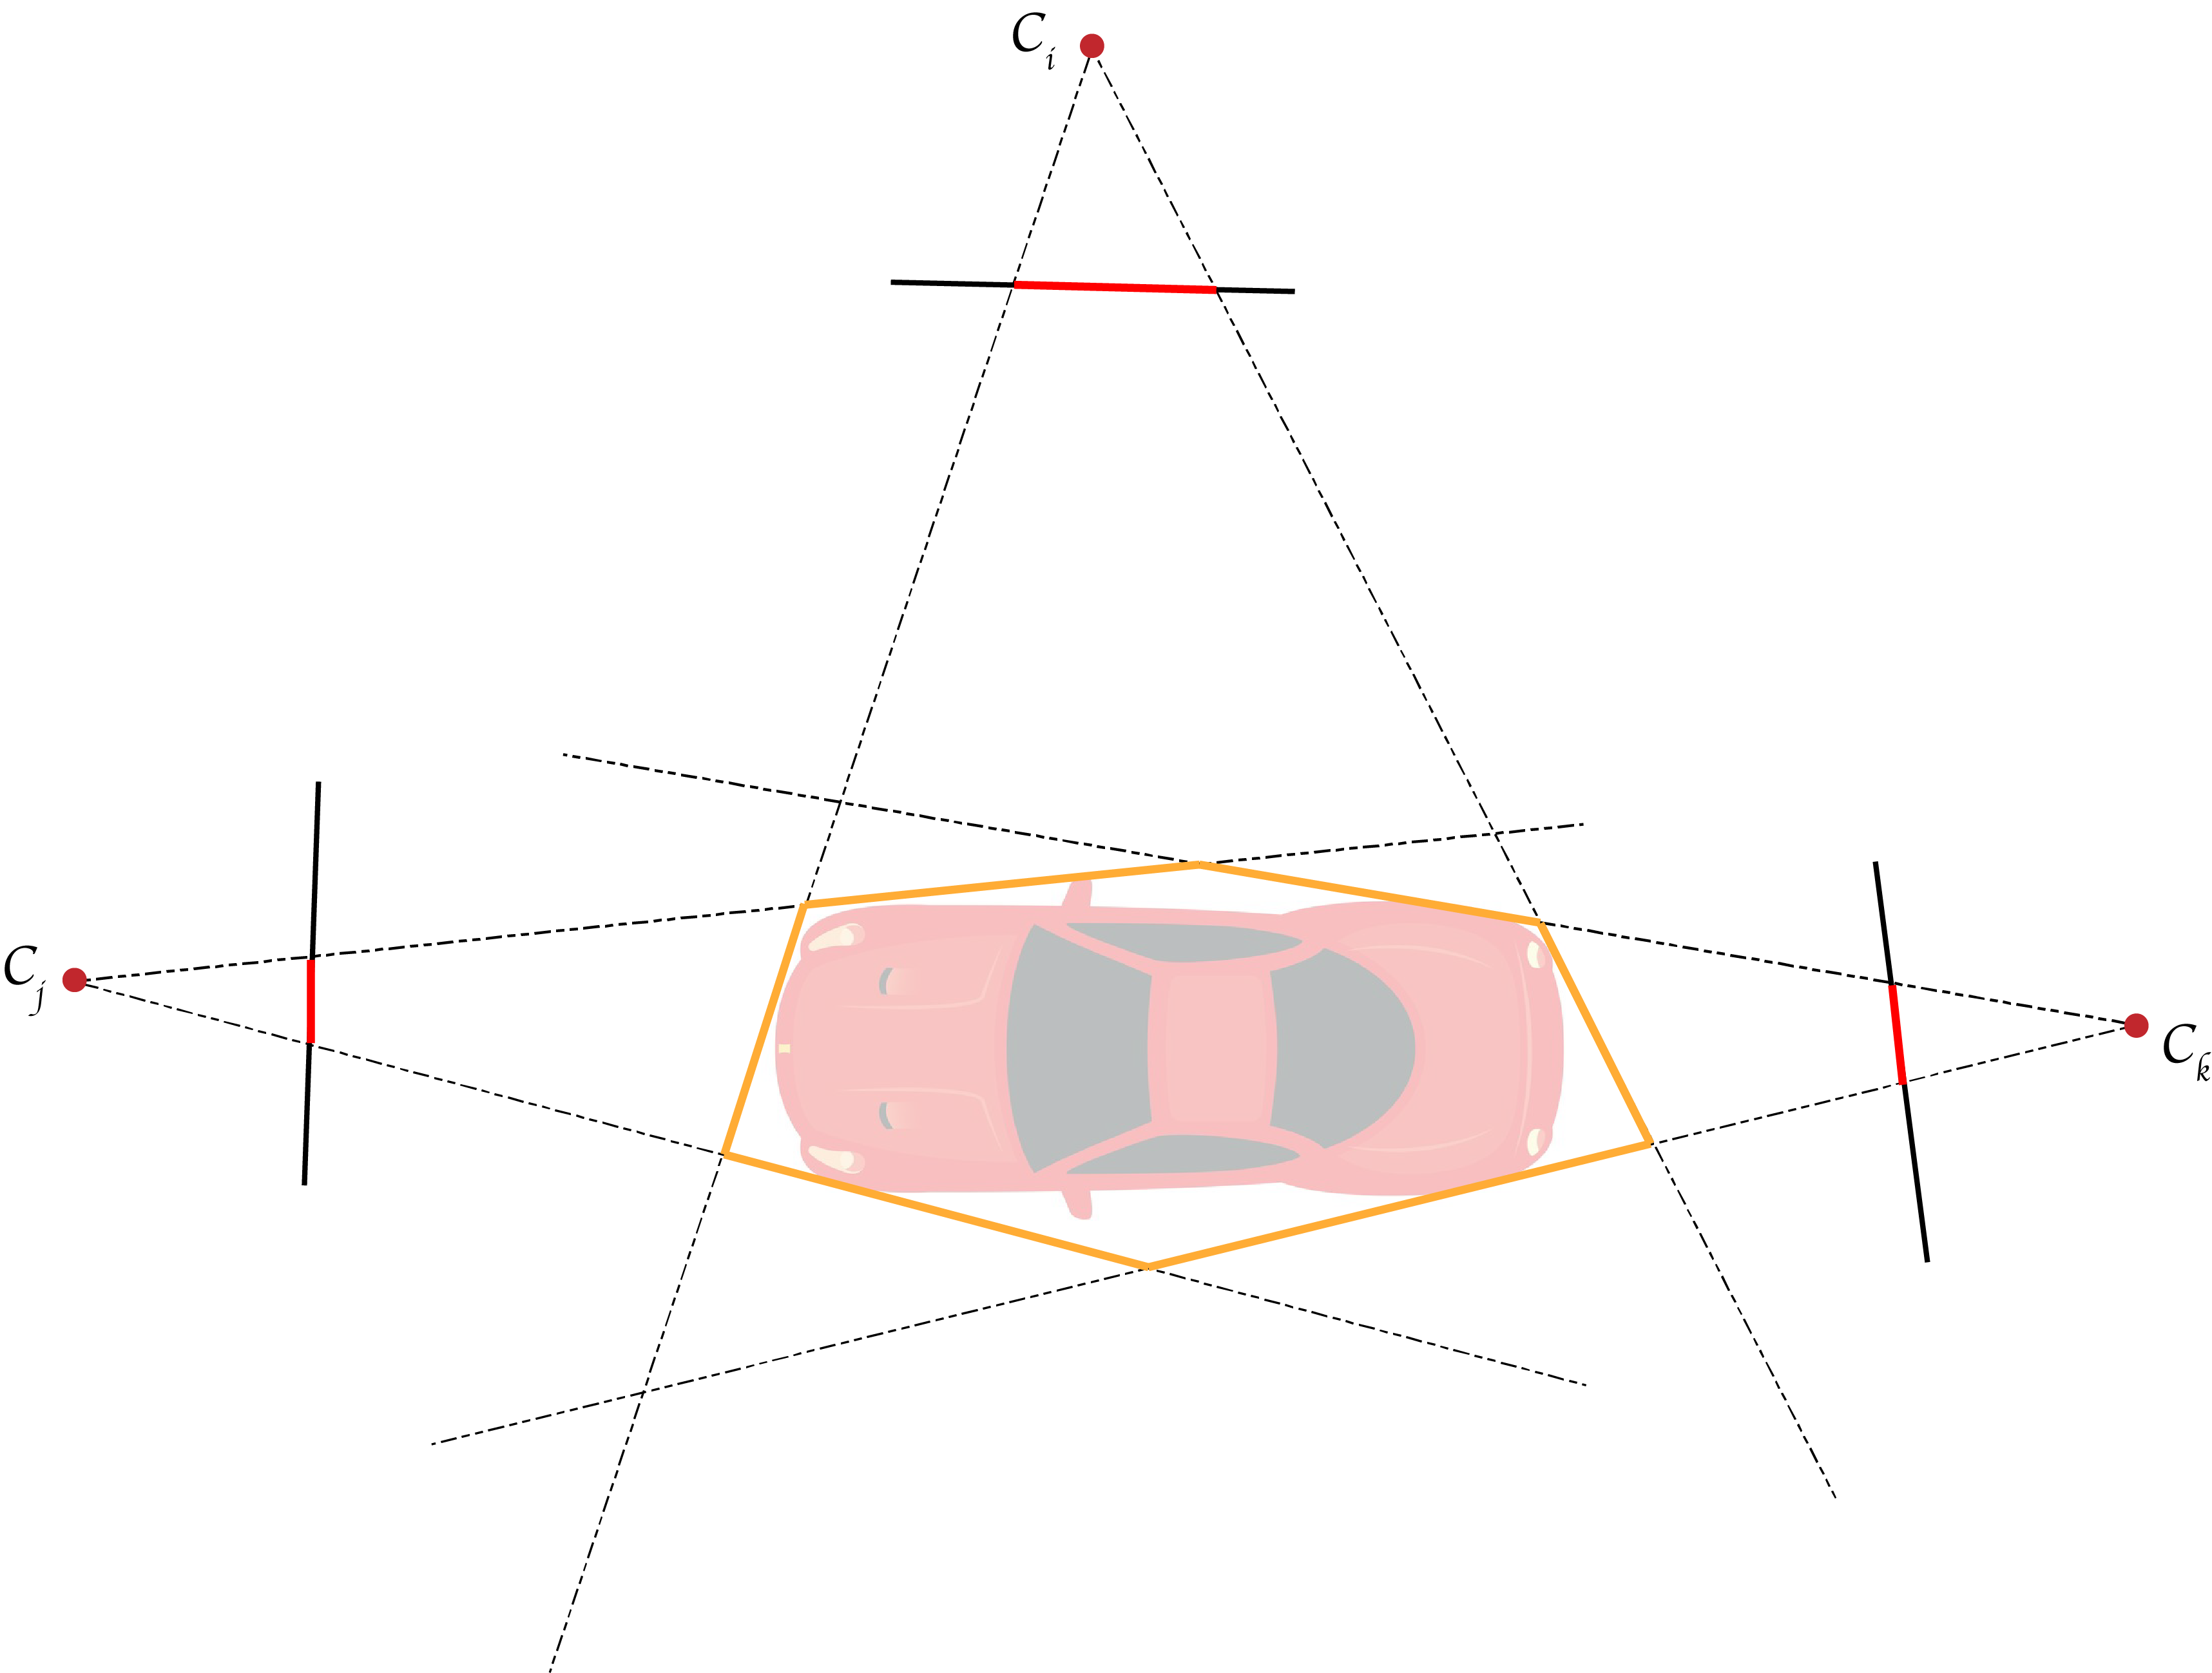
\includegraphics[width=\linewidth]{images/gaussiansplatting/visualhull-idea.png}
    \caption{\textbf{Overview idea}}
    \label{fig:gs-vh-concept}
  \end{subfigure}
  \quad % Space between the figures
  \begin{subfigure}[b]{0.48\linewidth}
    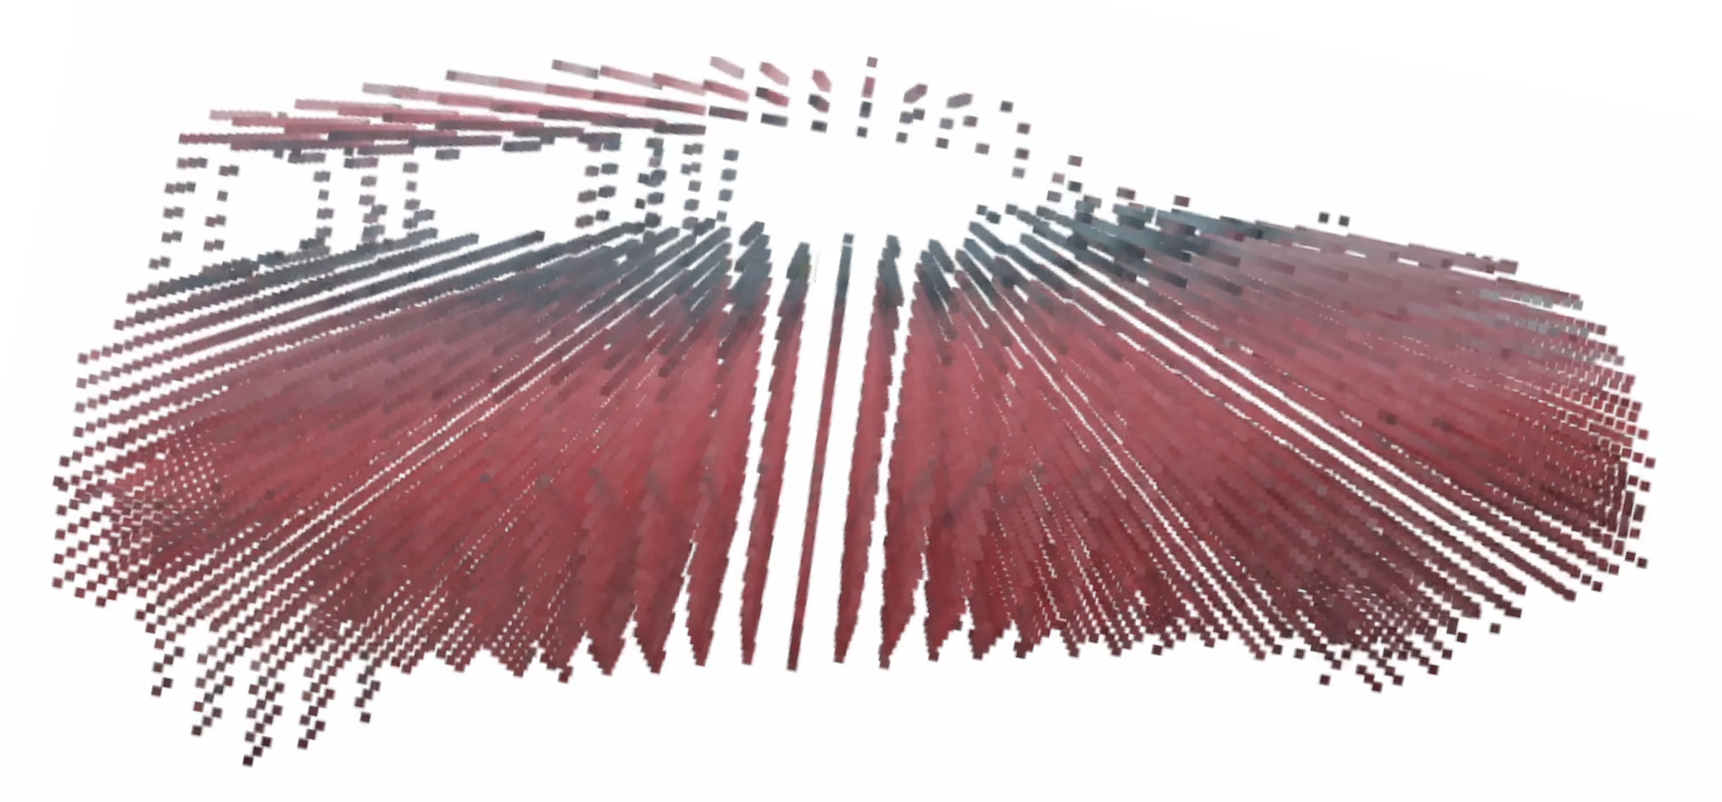
\includegraphics[width=\linewidth]{images/gaussiansplatting/visualhull-res.png}
    \caption{\textbf{Resulting hull}}
    \label{fig:gs-vh-result}
  \end{subfigure}
  \caption{\textbf{Visual hull concept.} A visual hull is here built as the intersection of three 3D bounding cones from the silhouette masks. Such hull is almost convex in case of our car scenario. One can  sample 3D points within the visual hull to build a new dense point cloud.}
  \label{fig:gs-homography-view3}
\end{figure}

We consider a novel point cloud method initialisation by leveraging upon a visual hull, a silhouette-from-motion \citep{baumgart1974geometric} based-concept. It only requires to get the posed images $\{I_{i},\pi_{i}\}_{i=1}^{N}$ and their corresponding binary silhouette masks. Figure \ref{fig:gs-vh-concept} illustrate the visual hull concept. 

We present on Algorithm \ref{alg:gs-vh} the pseudo code that generates such a visual hull point cloud. 

\begin{algorithm}[htpb!]
  \caption{Visual hull contruction}\label{alg:gs-vh}
  \SetKwInOut{Input}{input}
  \SetKwInOut{Output}{output}
  \SetKwInOut{Parameter}{parameter}
  \Input{Images $\mathcal{I}$, Silhouette mask $\mathcal{S}$}
  \Parameter{Intrinsic and extrinsic camera parameters $\pi=K[R|t]$}
  \Output{Visual hull-based point cloud $\mathcal{P}_{VH}$ } 
  \medskip
  \KwResult{$\mathcal{P}_{VH}$ can be densely sampled}
  \medskip
  $bbox \gets \mathbf{build3DBB}()$ \tcp*[l]{Create a vanilla 3D bounding boxe}
  $P_{3D} \gets \mathbf{sampleDensely}(bbox)$\hspace{.4cm}\textcolor{gray!80}{\# 
    [$N_{pts}$,3]} \tcp*[l]{Sample points in the BB}

   $P_{2D} \gets \mathbf{project}(P_{3D},\pi)$ \hspace{.4cm}\textcolor{gray!80}{\# 
    [$N_{pts}$,2]} \tcp*[l]{Reproject on image plane }
    
    $idx_{valid} \gets \mathbf{keepValidPoints}(P_{2D},\mathcal{M})$ \hspace{.4cm}\textcolor{gray!80}{\# 
    [$N_{pts}$,1]} \tcp*[l]{Boolean. 1 if valid, 0 otherwise}

    $P_{3D}^{(refined)} \gets P_{3D}[idx_{valid}]$ 

    $P_{VH} \gets \mathbf{setRGBcolor}(P_{3D}^{(refined)},P_{2D},idx_{valid},\mathcal{I})$ \tcp*[l]{Set RGB color to the point cloud through bilinear interpolation}
\end{algorithm}


\subsection{Viewing Direction}
Second bloc we get into consideration on top of the existing GS vanilla framework come from \ac{VDGS} \citep{malarz2023gaussian}. Core authors idea is to some extend mix concepts from both NeRF and GS to get the most of both framework, as depicted on Figure \ref{fig:gs-nerf}. 

\begin{figure}[htpb!]
  \centering
  \begin{subfigure}[b]{0.31\linewidth}
    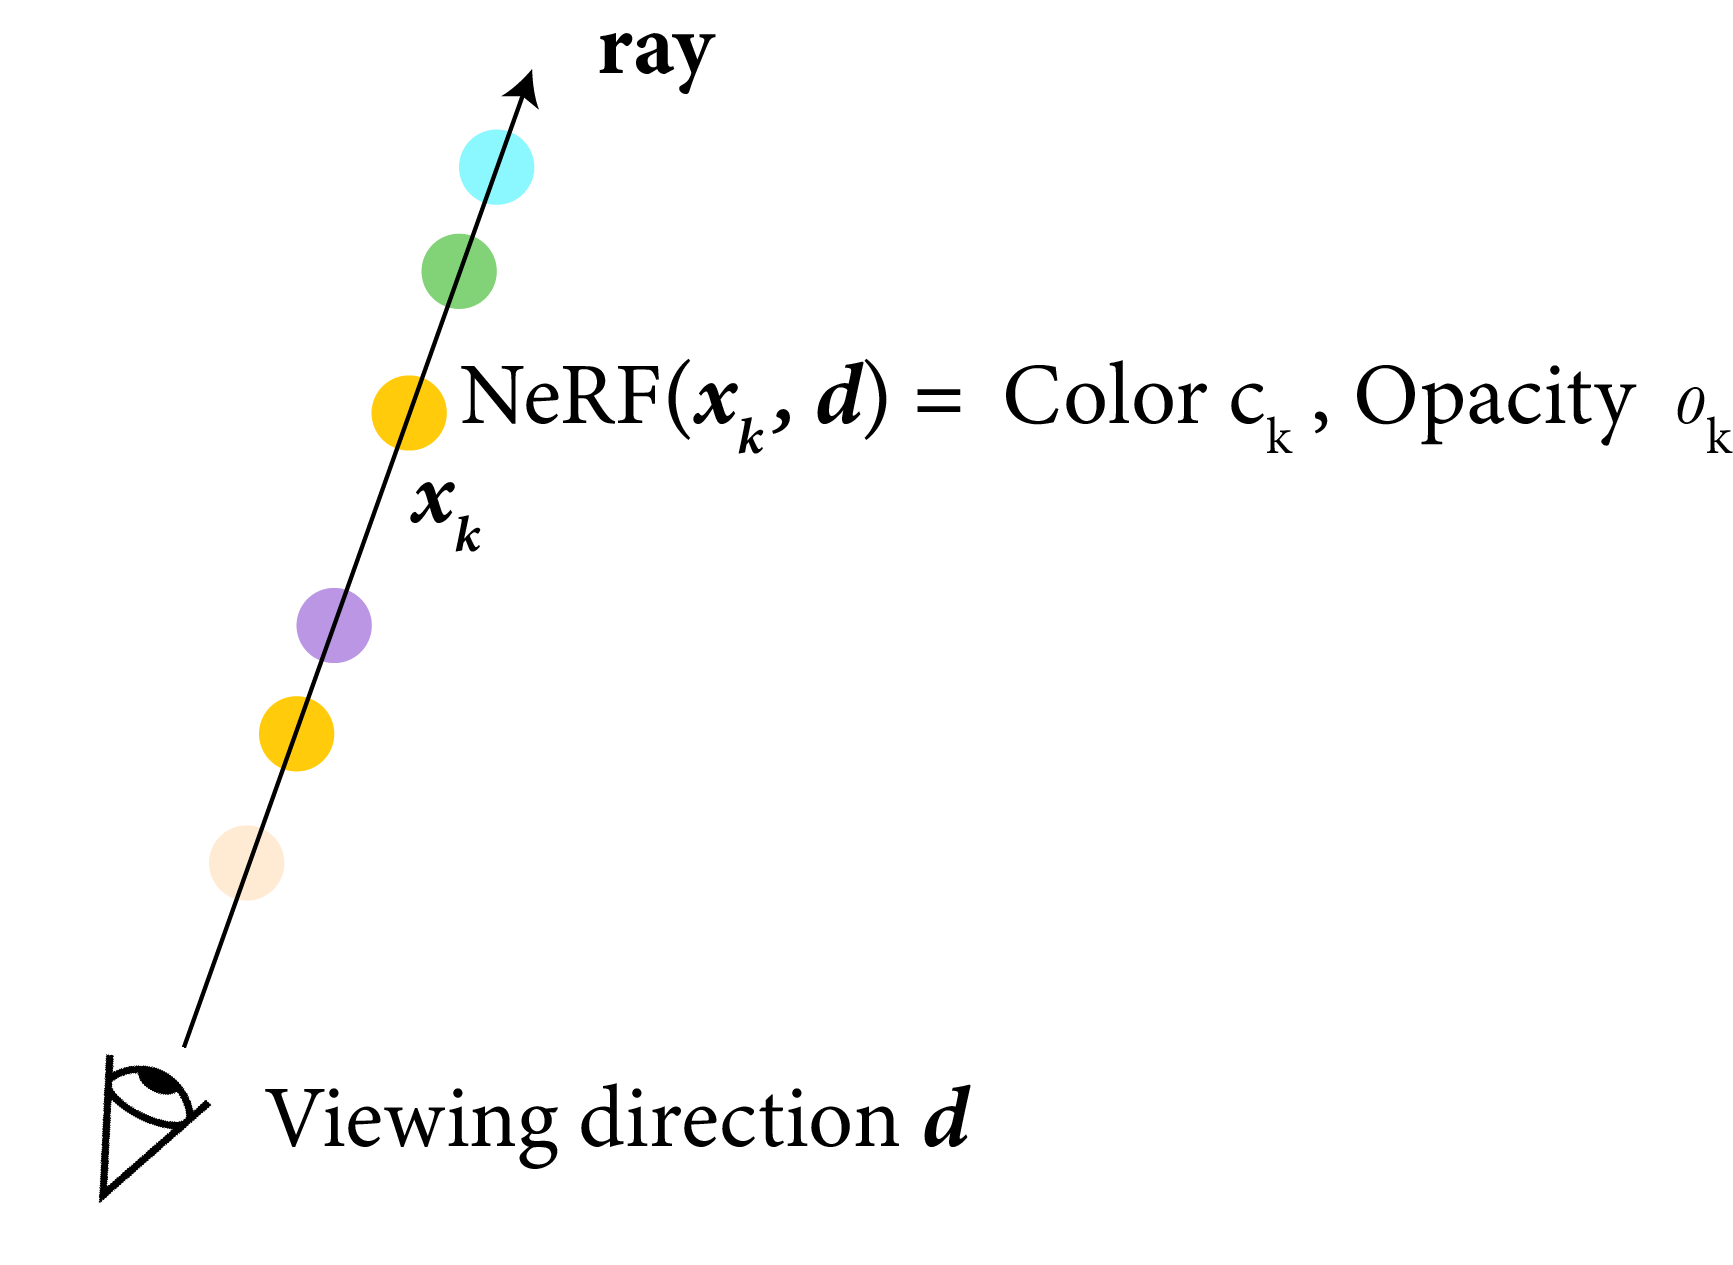
\includegraphics[width=\linewidth]{images/gaussiansplatting/nerf.png}
    \caption{\textbf{NeRF-based}}
    \label{fig:nerf-ray}
  \end{subfigure}
  \quad % Space between the figures
  \begin{subfigure}[b]{0.31\linewidth}
    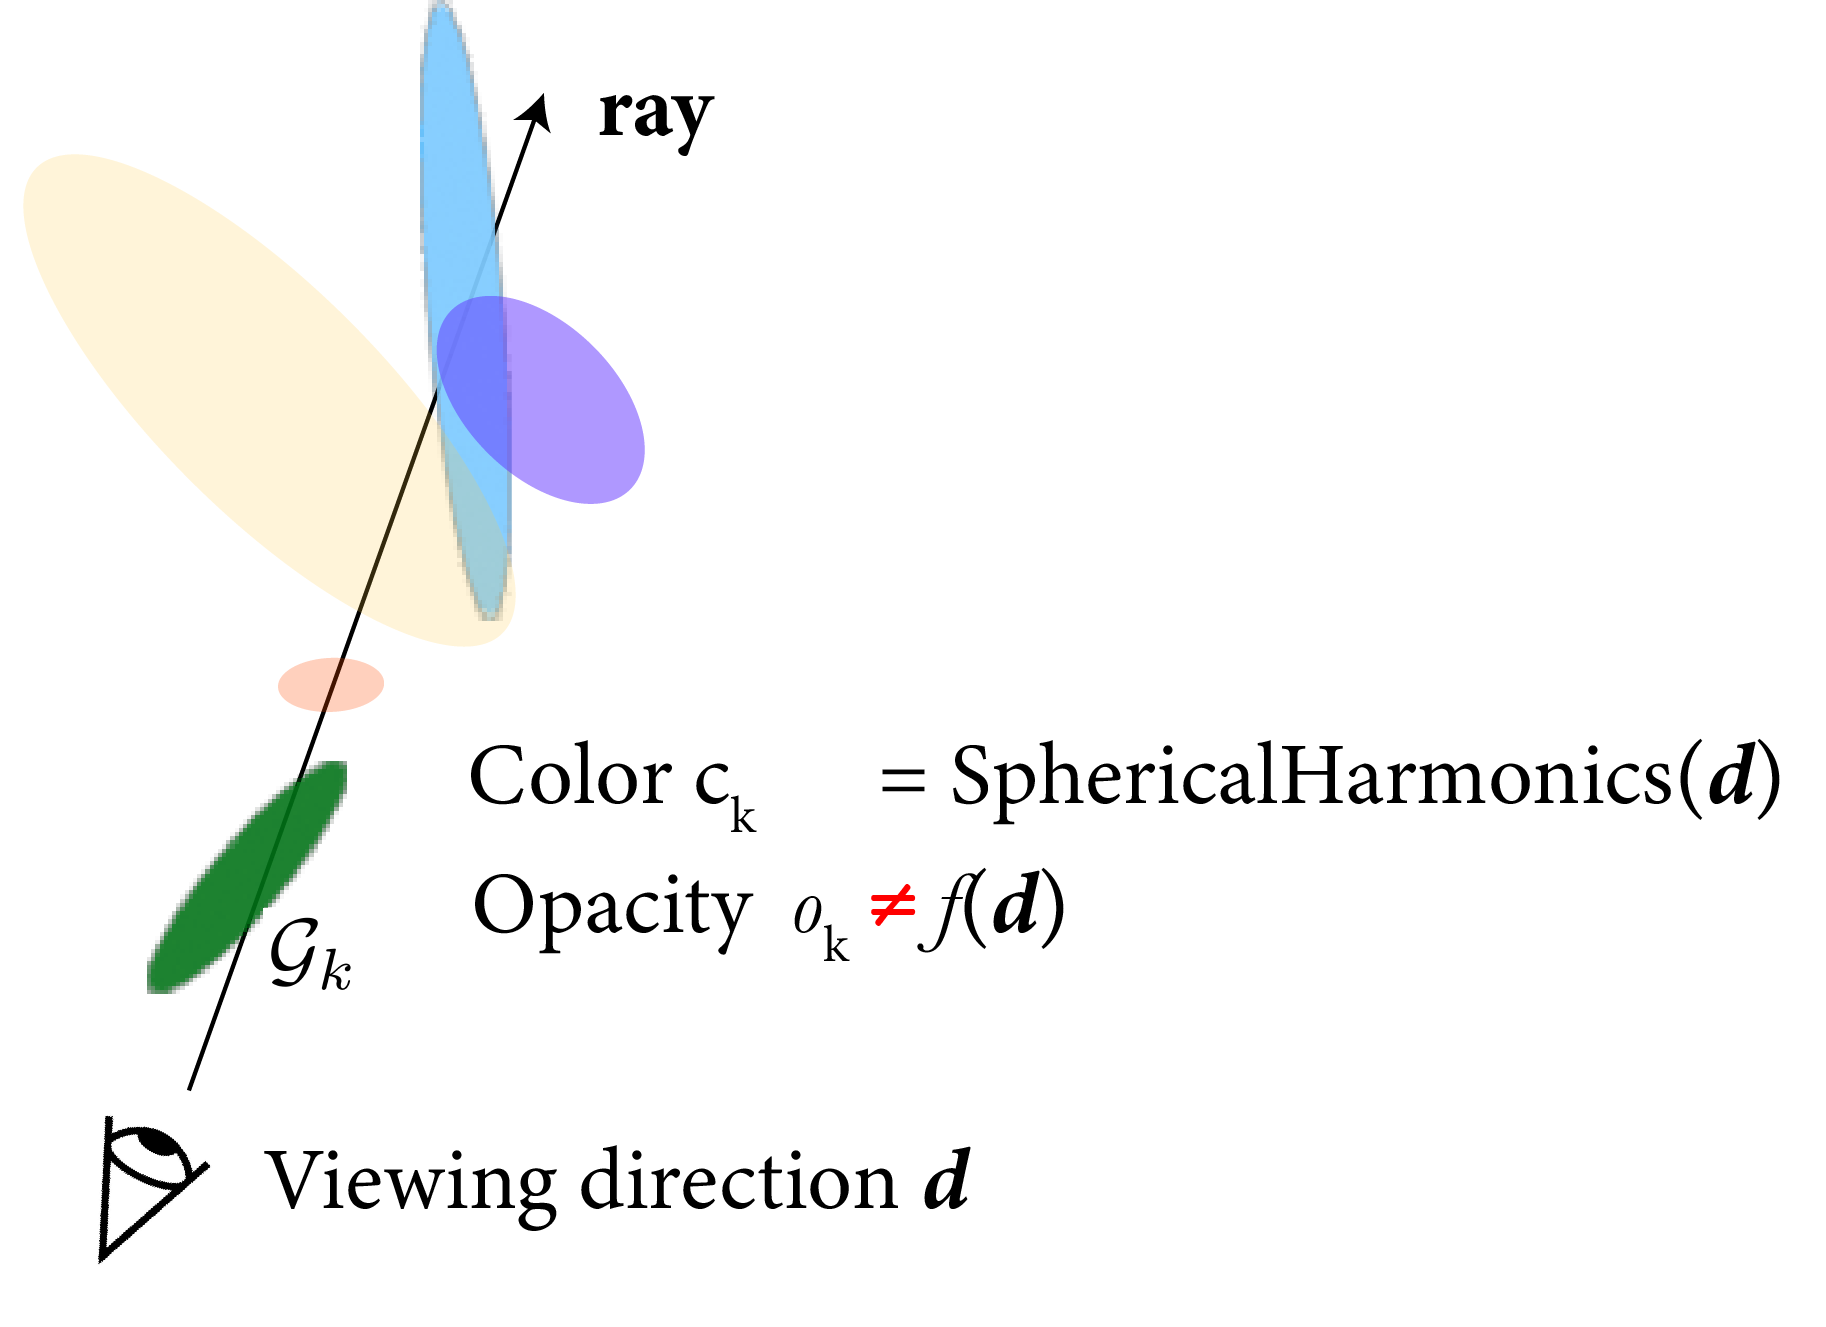
\includegraphics[width=\linewidth]{images/gaussiansplatting/gs_vanilla.png}
    \caption{\textbf{GS-based}}
    \label{fig:gs-ray}
  \end{subfigure}
  \quad % Space between the figures
  \begin{subfigure}[b]{0.31\linewidth}
    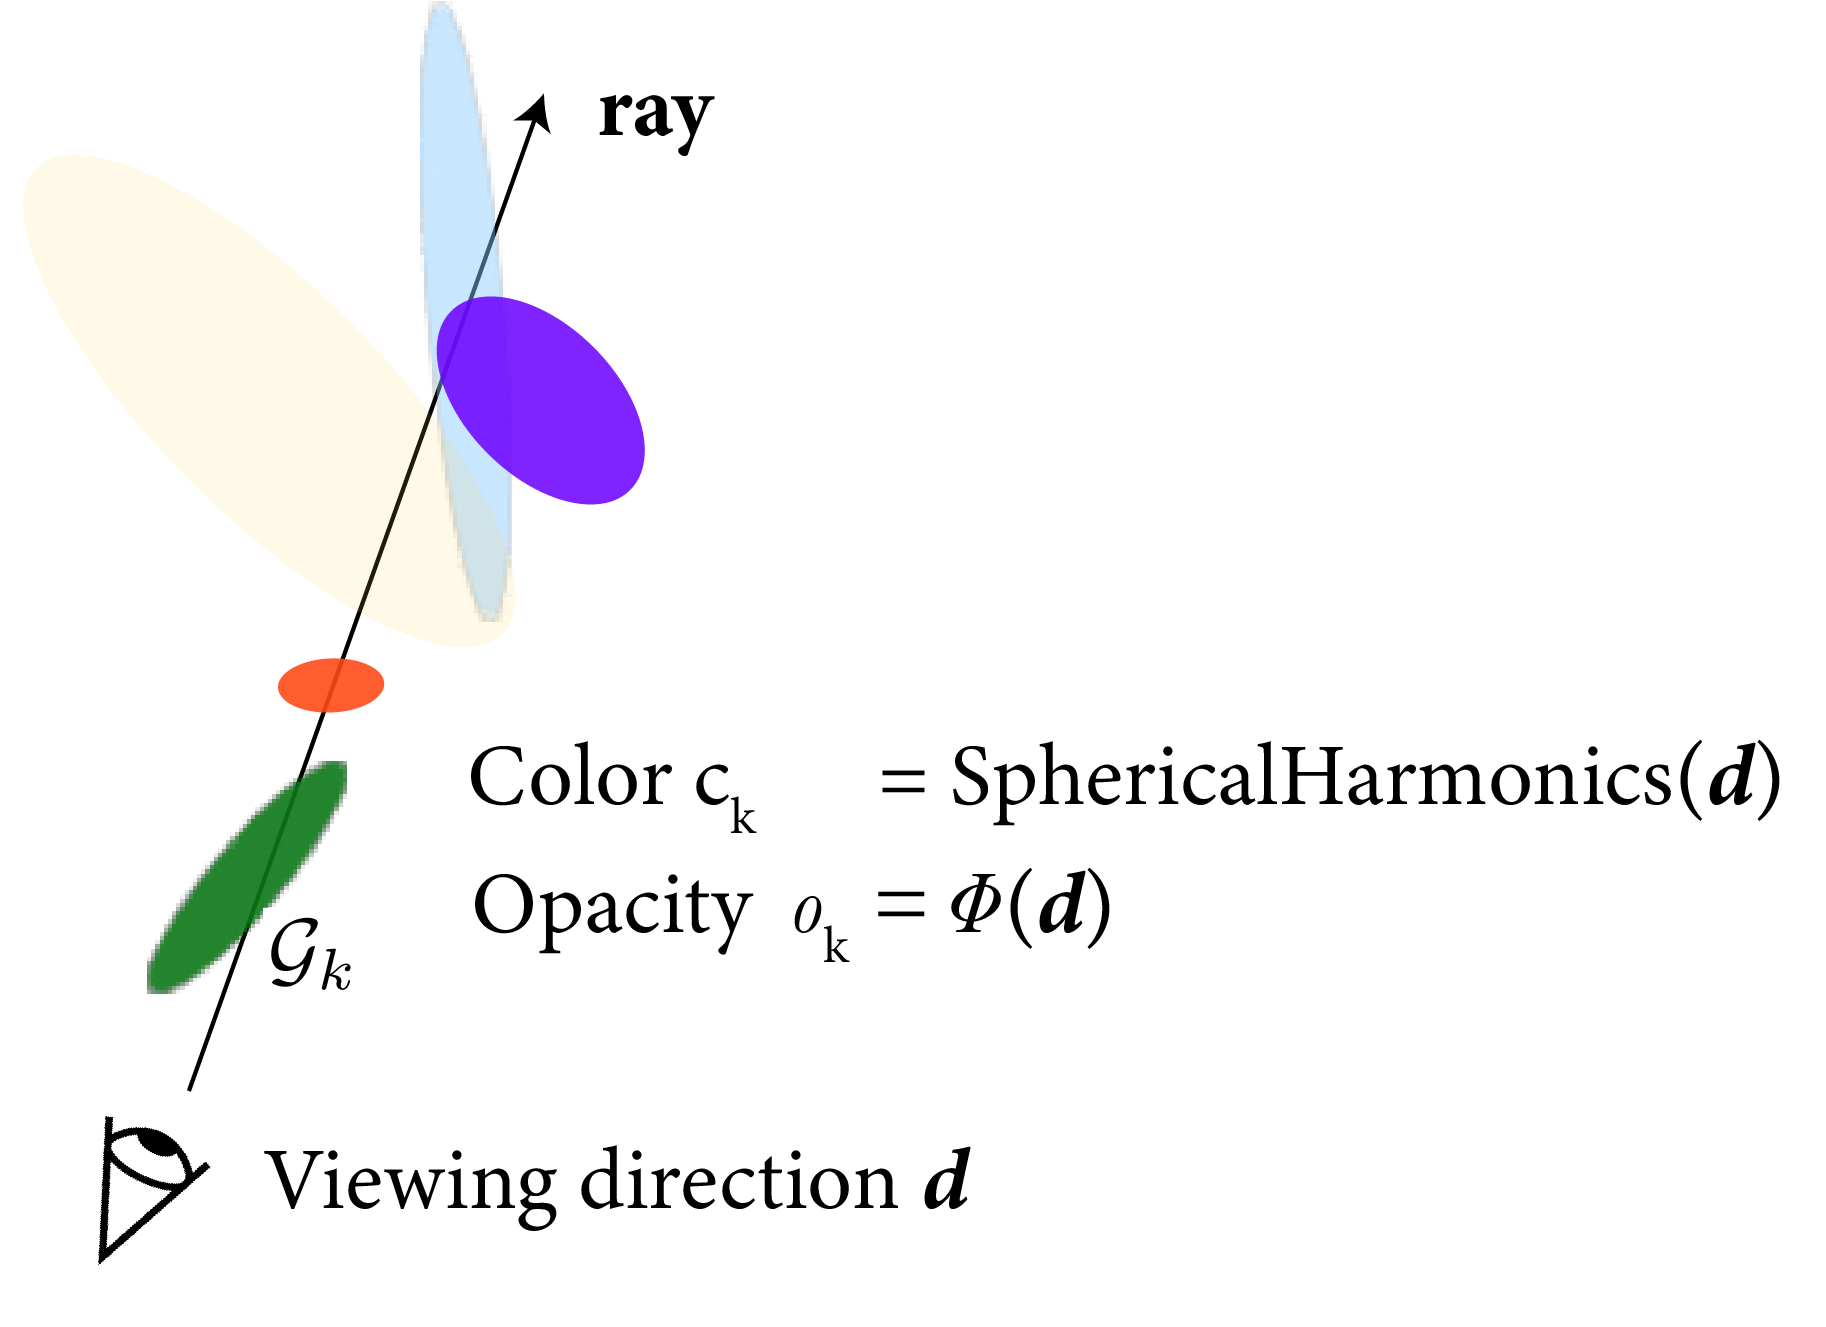
\includegraphics[width=\linewidth]{images/gaussiansplatting/gs.png}
    \caption{\textbf{Ours}}
    \label{fig:gs-ray}
  \end{subfigure}
  \caption{\textbf{Conceptual difference between NeRF and GS.} Neural radiance fields output color and opacity as a function of the viewing direction. Original \ac{GS} solely encodes view dependency through the \ac{SH} basis. Our modification allows to also output the opacity value of each primitive as a function of \textbf{d}.}
  \label{fig:gs-nerf}
\end{figure}

The trained 3D\ac{GS} scene remains expressed as a 3D gaussians cloud but authors introduced an additional \ac{MLP} that is going to output a corrective update on each gaussian opacity value. 

Indeed, primitive opacity originally does not depend on the viewing direction \textbf{d} we looking at during rasterization. Introducing such a \ac{MLP}, termed $\Phi$, therefore aims to adjust gaussian transparency: 

\begin{equation}
\Delta o^{(k)} = \Phi(\Sigma_{3D}^{(k)},c^{(k)},\textbf{d}) 
\end{equation}

so that the final corrected opacity is expressed as: 

\begin{equation}
o^{(k)} \gets \Delta o^{(k)}(\textbf{d}) \times o^{(k)} 
\end{equation}

This novel view-dependent opacity allow to better handle surface light reflections as well as transparent regions on car windows. It worth noting the alpha-blending equation introduced in equation (\ref{eq:gs-alpha-blending}) remains unchanged to get the final rendered pixel color.

Such a lightweight \ac{MLP} $\Phi$ thus highly improve the light reflections and windows transparency issue we often encounter in our car scenes. In-depth quantitative figures as well as visual insights of such an opacity view dependency impact are presented in section \ref{sec:exp-gs}. 

\subsection{PixGS ADC}
\label{gs:pixgs-adc}
Our latest improvement of the vanilla GS framework is directly link to the way gaussians are splited and cloned during the \ac{ADC} procedure. We extensively leverage upon PixGS \citep{zhang2024pixelgs} to update the densification formulation.  

Original \ac{ADC} strategy has several inner limitations in its current form: 
\begin{itemize}
    \item Per-pixel gradient involved in $\frac{\partial L_{\pi}}{\partial \mu^{k,\pi}_{ndc,x}}$ and $\frac{\partial L_{\pi}}{\partial \mu^{k,\pi}_{ndc,y}}$  have different directions. It lead to gradient collision, where the magnitude of $\frac{\partial L_{\pi}}{\partial \mu_{k}^{\pi}}$ does not reach densification threshold, even though it should. 
    \item Setting the two thresholds involved in the densification process is not intuitive: optimal threshold values might vary from a scene to another one and need to be adjusted empirically.
    \item There is no explicit control regarding the total number of gaussians a scene can reach, leading to potential out-of-memory \ac{GPU} issues during training.
\end{itemize}

An initial sparse point cloud areas lead to large ellipsoids primitives during initialisation as soon as gaussians axes length are set based on the nearest neighboring points. Large gaussians are thus involved in the loss computation from too many viewpoints. However, summing gradients across numerous viewpoints and pixels with varying directions can reduce the overall magnitude that \ac{ADC} is tracking for densification. Such a behaviour is illustrated on Figure \ref{fig:adc-limitation}. 

\begin{figure*}[htbp!]
    \center
  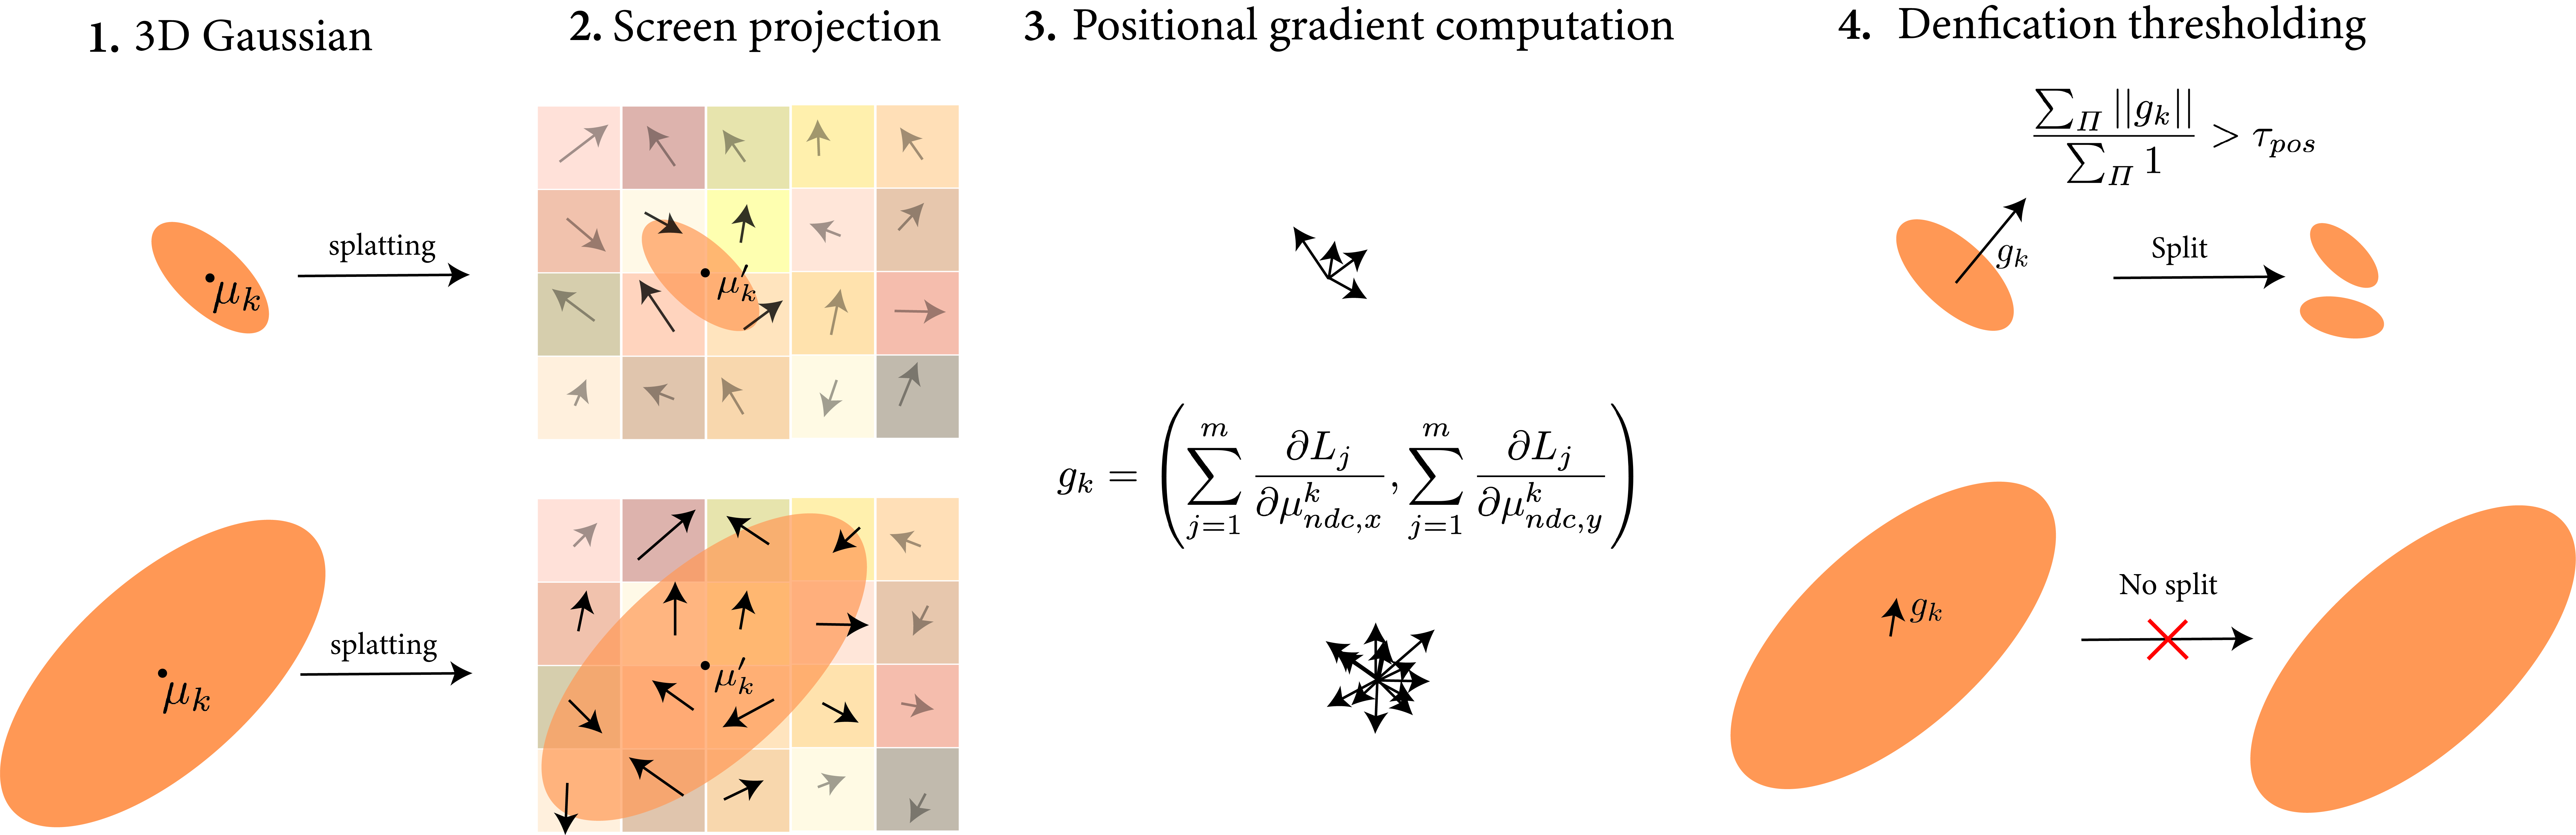
\includegraphics[width=\linewidth]{images/gaussiansplatting/adc_limitation.png}
  \caption{\textbf{ADC gradient collision.} It might occurred that large gaussians ends with low magnitude gradient, preventing the densification to happen.}
  \label{fig:adc-limitation}
\end{figure*}



To ease notation, we discard viewpoint $\pi$ and denote: 

\begin{equation}
\label{eq:grad-inter}
    g_{k,x} = \frac{\partial L}{\partial \mu^{k}_{ndc,x}} = \sum \limits_{j=1}^{m} \frac{\partial L_{j}}{\partial \mu^{k}_{ndc,x}} 
\end{equation}

the x-axis gradient, with the per-pixel gradient expression: 

\begin{equation}
\label{eq:perpix-grad}
\frac{\partial L_{j}}{\partial \mu^{k}_{ndc,x}} = \sum \limits_{l=1}^{3} \frac{\partial L_{j}}{\partial c_{l}^{j}}\times \frac{\partial c_{l}^{j}}{\partial \alpha_{k}^{j}} \times \frac{\alpha_{k}^{j}}{\partial \mu^{k}_{ndc,x} }
\end{equation}

where $c_{l}^{j}$ refers to the color of the $l^{th}$ channel of the pixel $j$. The three different partial derivatives from equation \eqref{eq:perpix-grad} might have different signs, affecting $\frac{\partial L_{j}}{\partial \mu^{k}_{ndc,x}}$ from equation (\ref{eq:grad-inter}). Complete proof can be found in appendix section \ref{appendix:sign-gradient}. The more we sum over a large number of pixel, the more likely $\frac{\partial L}{\partial \mu^{k}_{ndc,x}}$ is prone to get closed to zero, preventing $\nabla_{\mu_{k}}L$ to be higher than $\tau_{pos}$ during the iteration cycle, as shown on Figure \ref{fig:adc-limitation}. 

PixGS tackles this gradient collision by re-weighting equation (\ref{eq:adc-original}) with the number of pixels $m_{k}$ covered by each primitives $\mathcal{G}_{k}$: 

\begin{equation}
\frac{\sum \limits_{\pi \in \Pi} m_{k}^{\pi} ||\frac{\partial L_{\pi}}{\partial \mu_{k}}||}{\sum \limits_{\pi \in \Pi}m_{k}^{\pi}} > \tau_{pos}
\label{eq:adc-pixgs}
\end{equation}

PixelGS re-weighting strategy is illustrated on Figure \ref{fig:pixgs-adc}. 


\begin{figure*}[htbp!]
    \center
  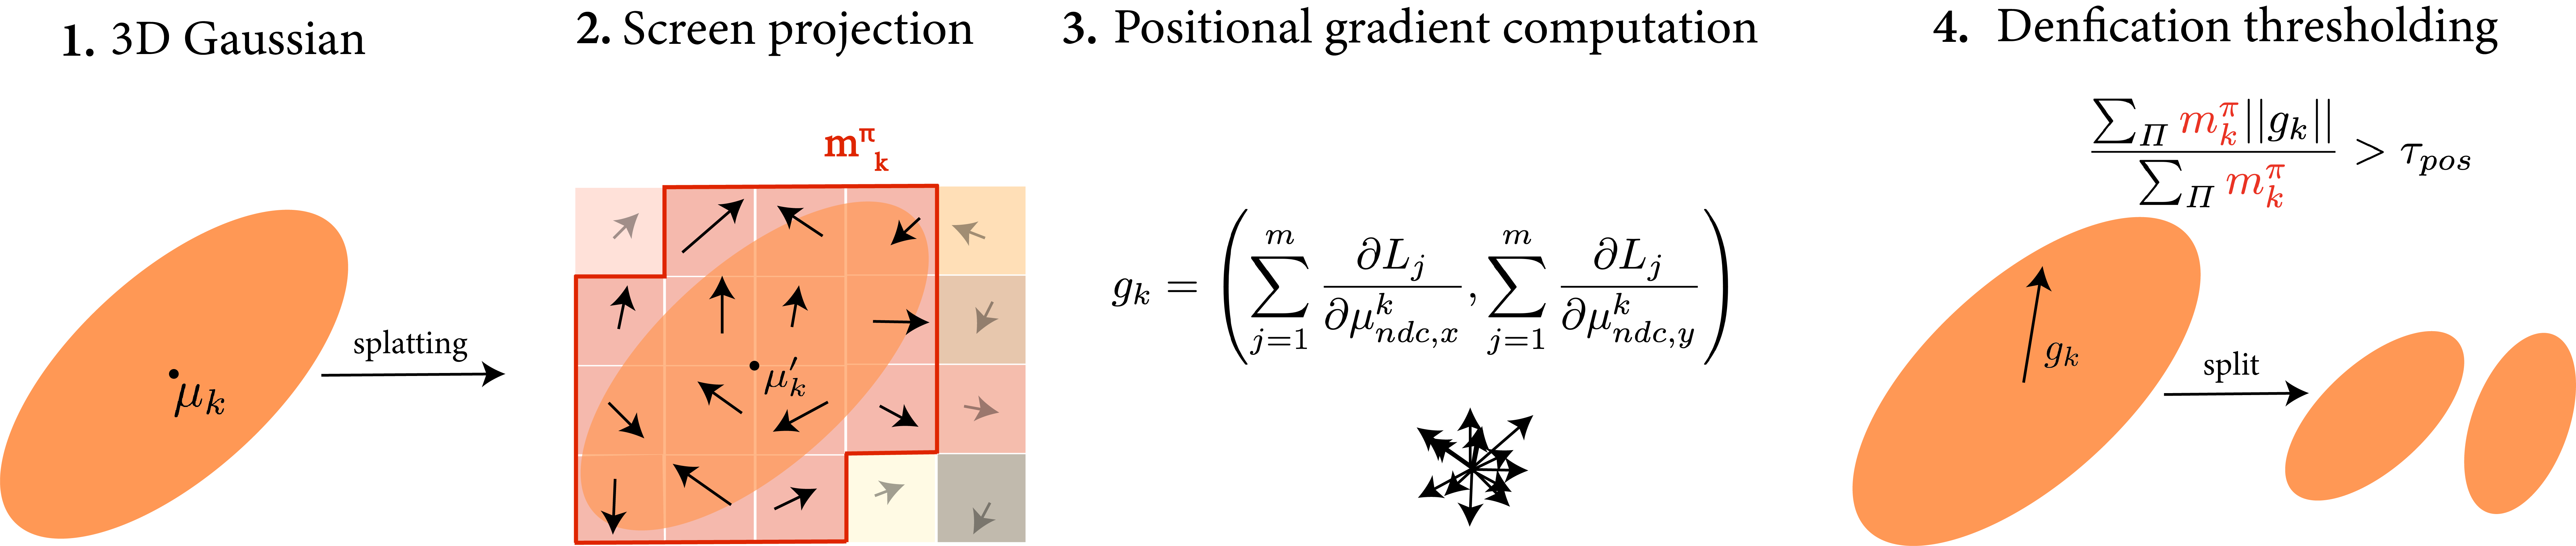
\includegraphics[width=\linewidth]{images/gaussiansplatting/pixgs_implem_improvement.png}
  \caption{\textbf{PixGS ADC correction.} By accounting on the number of pixel covered by a primitive, large gaussians with a large gradient are more likely to reach the density threshold $\tau_{pos}$.}
  \label{fig:pixgs-adc}
\end{figure*}


\section{Experiments}
\label{sec:exp-gs}

As our work has to be framed within an industrial system, all presented results come from a unique scene made of the 36 views and depicted on Figure \ref{fig:all_views}. These images exactly matches the type of scene that a client might send to Meero for \ac{AI} processing.

\begin{figure*}[htpb!]
  \center
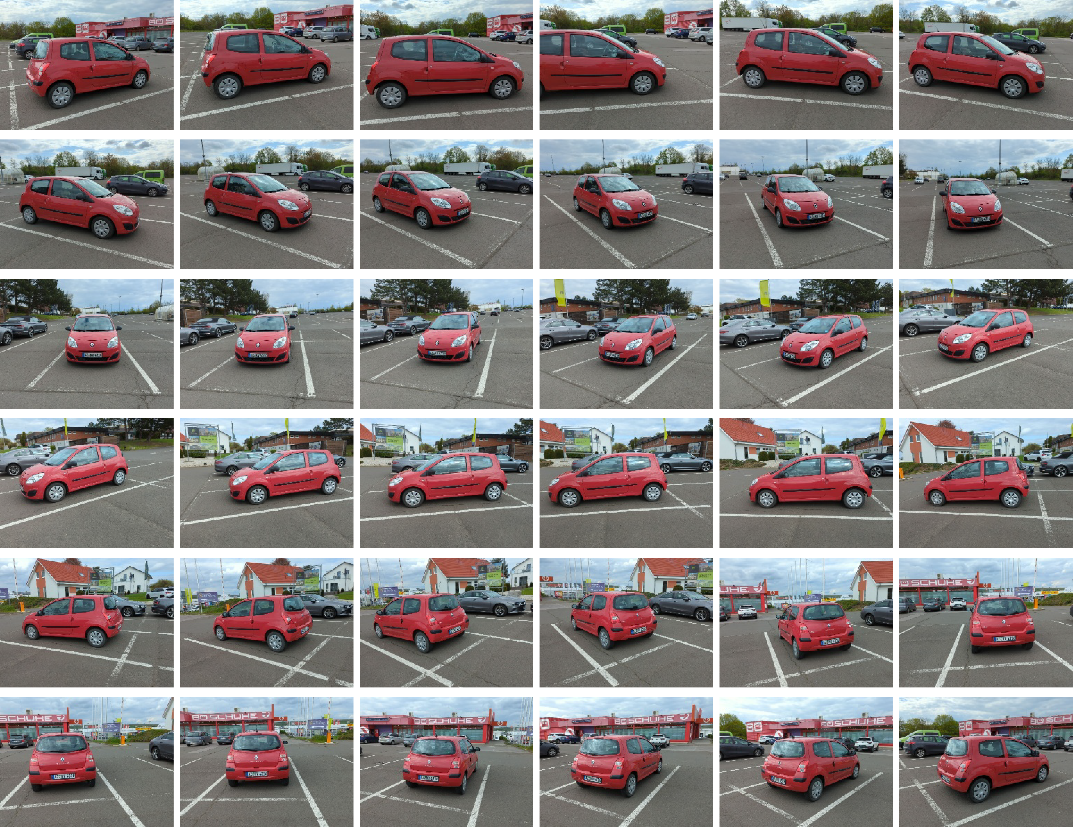
\includegraphics[width=.9\linewidth]{images/gaussiansplatting/original_scene.png}
\caption{\textbf{36 views $360^{\circ}$ spin scene.} Images has been acquired with a mobile device at $1500\times 2000$ resolution. As observed, car distance from the camera is inconsistent across viewpoint.}
\label{fig:all_views}
\end{figure*}

We give visual insights and quantitative figures in this section to highlight how each of the three modules we added to our \ac{GS} system consistently improved the rendering. 

\subsection{Viewing Direction}

Additional \ac{MLP} $\Phi$ that was added to our \ac{GS} pipeline significantly improves transparent areas (such as windows) and highly specular regions. We present a side-by-side comparison on Figure \ref{fig:gs-vh}. 

\begin{figure}[htb!]
  \centering
  \begin{subfigure}[b]{0.48\linewidth}
    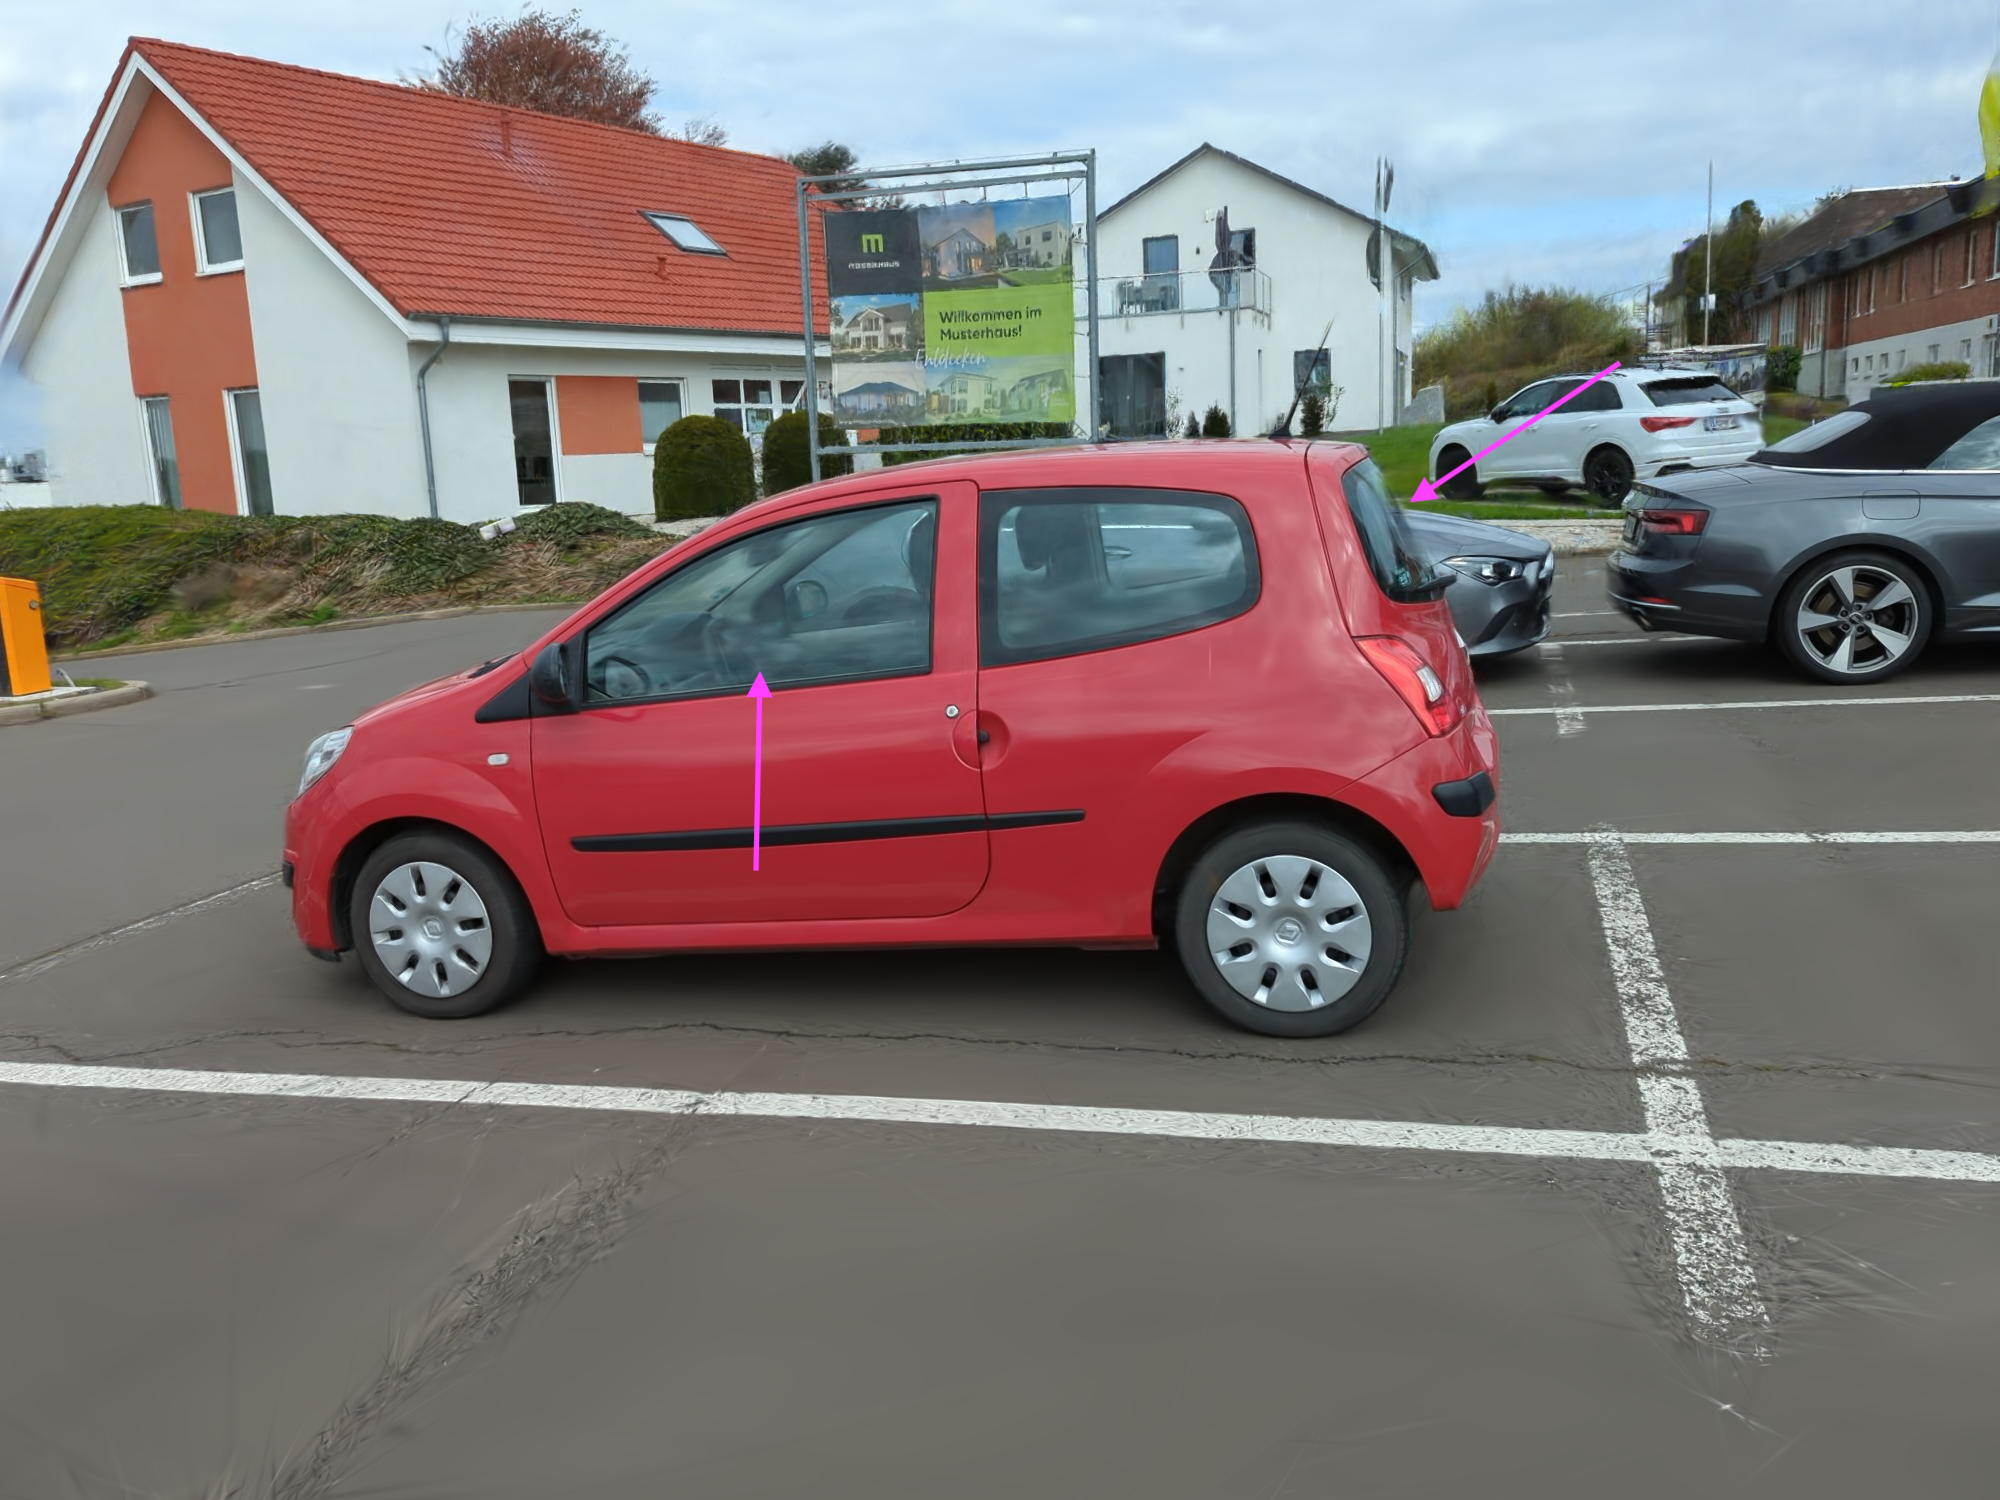
\includegraphics[width=\linewidth]{images/gaussiansplatting/00023-gs.png}
    \caption{\textbf{Vanilla GS rendering view}}
    \label{fig:view3}
  \end{subfigure}
  \quad % Space between the figures
  \begin{subfigure}[b]{0.48\linewidth}
    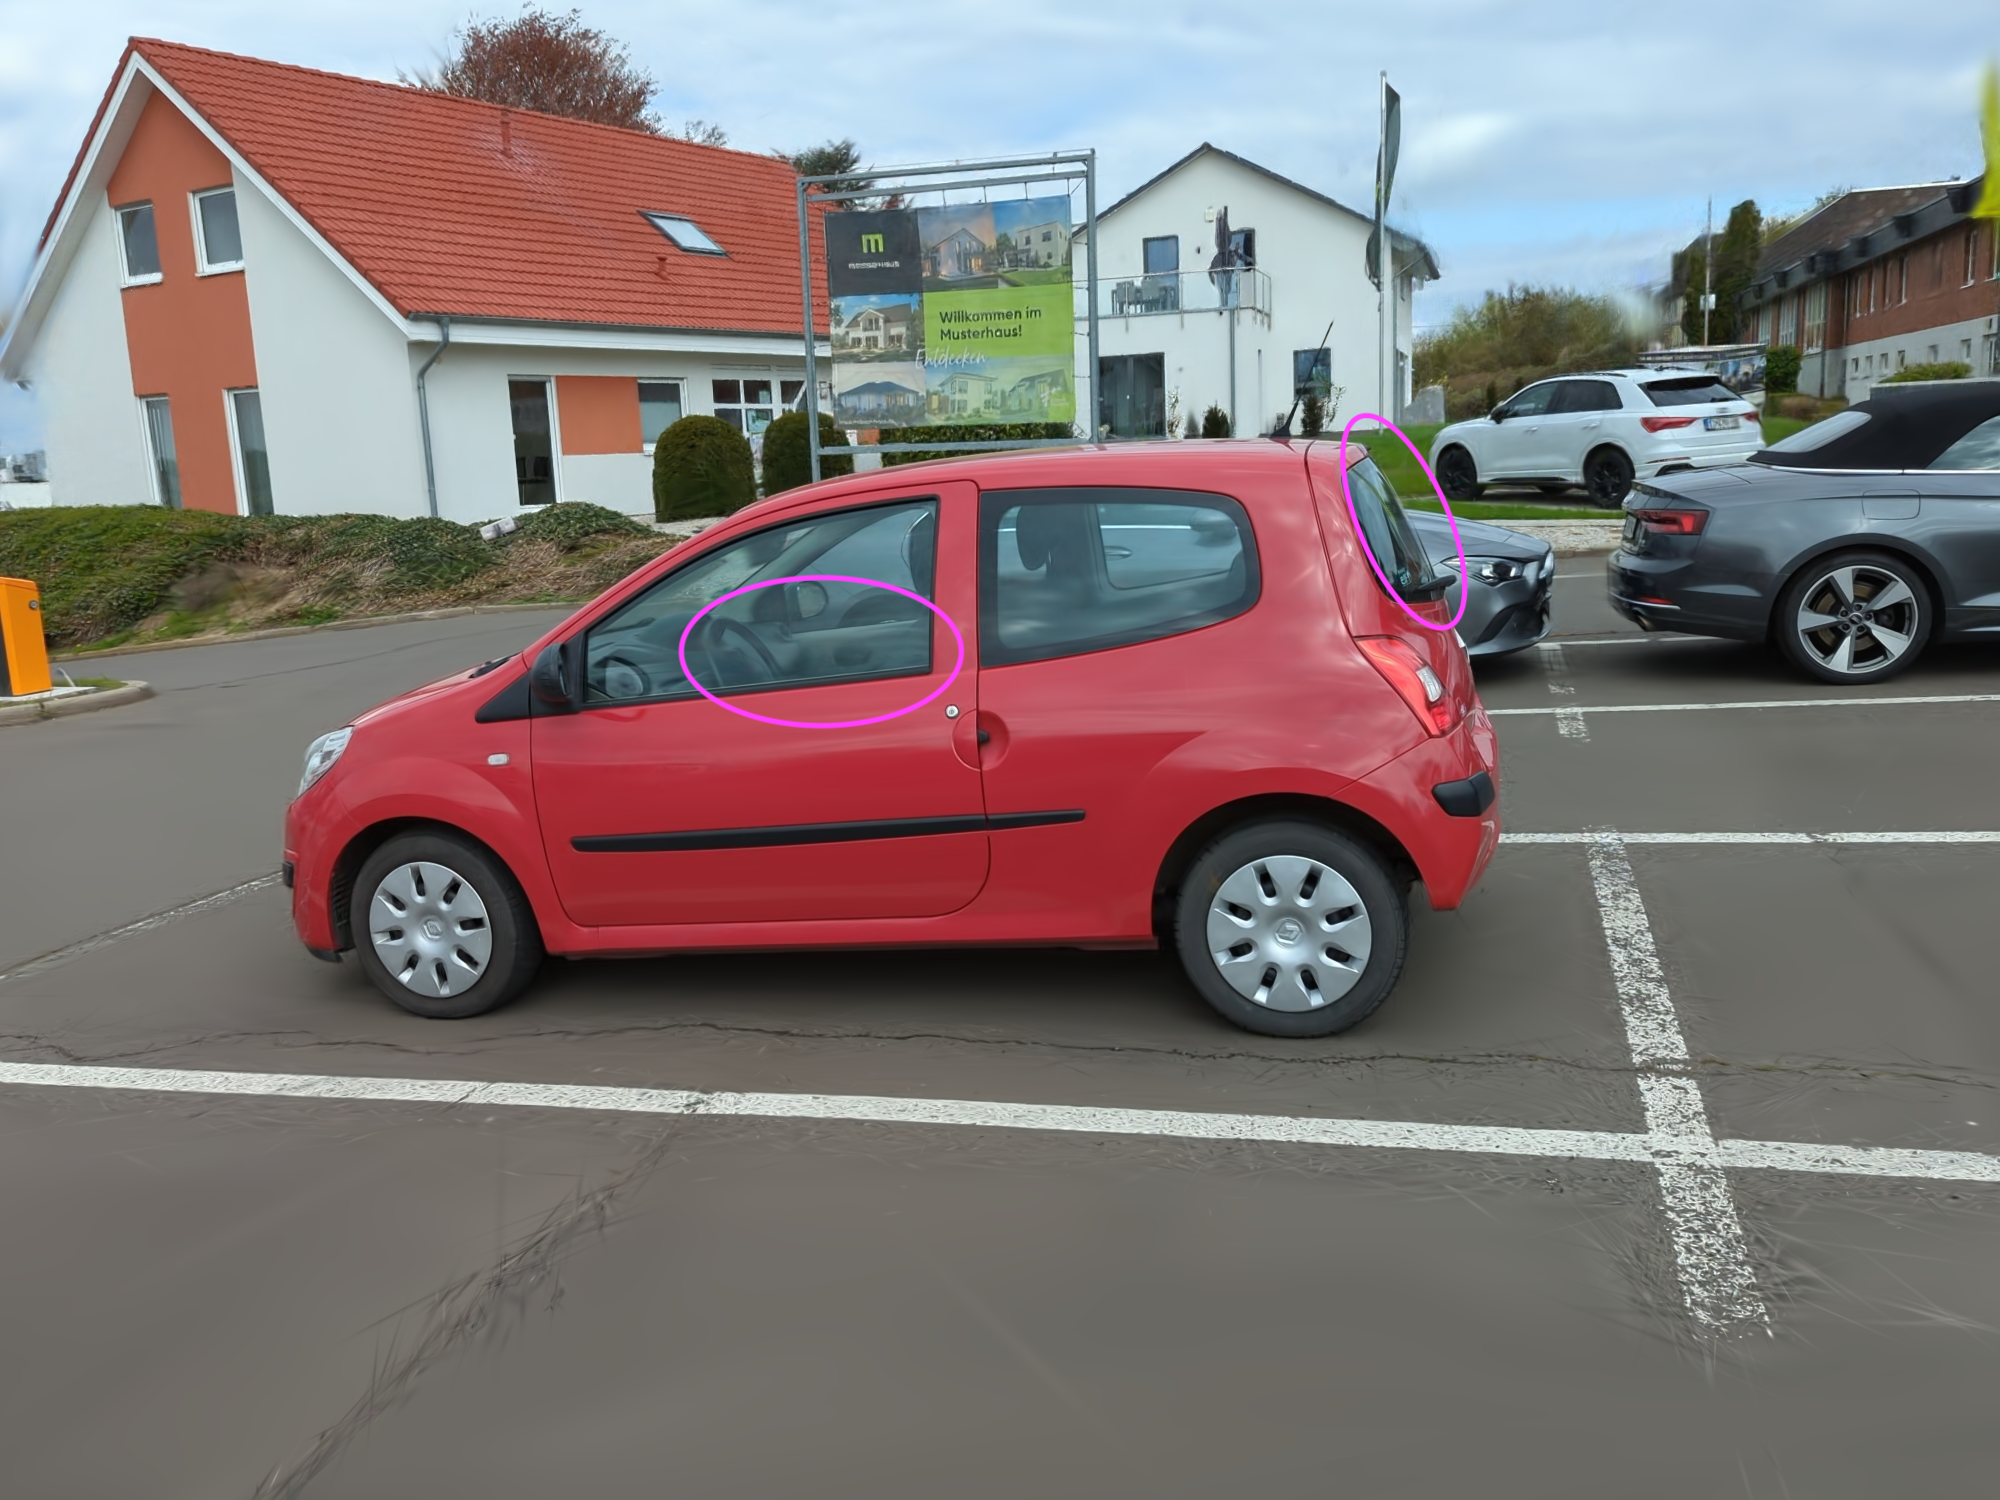
\includegraphics[width=\linewidth]{images/gaussiansplatting/00023-gs-vd.png}
    \caption{\textbf{With Viewing Direction MLP}}
    \label{fig:gs-view3-gs}
  \end{subfigure}
  \caption{\textbf{Viewing Direction influence.} Whereas vanilla 3D\ac{GS} struggles with reflective and transparent regions, adding such a \ac{MLP} before the rasterization significantly improve rendering results. }
  \label{fig:gs-vh}
\end{figure}


\subsection{Visual hull} 

We present on Figure \ref{fig:gs-vishull-comp} three renderings of the same view but from three different trainings. First scene was trained with the original point cloud produced by the COLMAP algorithm, second with the visual hull point cloud while the latest one uses merged COLMAP and visual hull point cloud.   

\begin{figure*}[htb!]
  \center
\includegraphics[width=\linewidth]{images/gaussiansplatting/vishull_ablation.png}
\caption{\textbf{Point cloud initilization influence.} The scene initialized with the merged two points clouds benefits from the best of both COLMAP and visual hull properties: the background is better rendered thanks to the COLMAP points while the car itself has more intricate details.}
\label{fig:gs-vishull-comp}
\end{figure*}

COLMAP based rendering yields a satisfying result, even though some inner details are missed. The visual hull based initialization method produce sharper results in the car, but floaters are rendered on the roof the car. Merging the two point cloud \textit{(right)} allows to get the best of both configuration. 

These visual improvement on the rendered views are quantitatively confirmed through the whole training set with the three metrics we used to assess the rendering quality. Results are gathered on Table \ref{table:gs-vh-influence}. Associated figures highlight a phenomena that is visible on Figure \ref{fig:gs-vishull-comp}: as soon as no points are affected in the background regions at the initialisation stage with the visual hull configuration, background rendering quality of the 3D\ac{GS} scene is poor compared to its  \textit{COLMAP} based counterpart. Such a limitation is quantatively confirmed on Table \ref{table:gs-vh-influence}: results from the visual hull configuration are better when metrics are only computed on the car. 
\begin{table}[htp!]
  \caption{\textbf{VisualHull influence.} Quantitative results how influenciable the original point cloud can be on the GS rendering performance.}
  \label{table:gs-vh-influence}
  \begin{adjustbox}{width=\linewidth}
  \begin{tabular}[h]{c||ccccccc}
  \hline
   PC initialization & \multicolumn{3}{c}{Full Image} & \multicolumn{3}{c}{Car only} \\
   &  SSIM ($\uparrow$) & PSNR ($\uparrow$) & LPIPS ($\downarrow$) & SSIM ($\uparrow$) & PSNR ($\uparrow$) & LPIPS ($\downarrow$)\\
  \hline
  COLMAP \textit{only} & 0.808 & 29.163 & 0.318 & 0.983 & 40.917 & 0.031\\
  VisualHull \textit{only} & 0.764 & 27.254 & 0.373 & 0.980 &   39.271 & 0.035 \\
  COLMAP + VisualHull & \textbf{0.810} & \textbf{29.288} & \textbf{0.314}  & \textbf{0.984} & \textbf{41.249}   & \textbf{0.030} \\
  \hline 
  \end{tabular}
  \end{adjustbox}
  \end{table}

\subsection{PixGS ADC} 

We finally highlight the positive impact a clever \ac{ADC} have on the final rendered views. Qualitative results are shown on Figure \ref{fig:gs-pigs}. 

\begin{figure}[htb!]
  \centering
  \begin{subfigure}[b]{0.45\linewidth}
    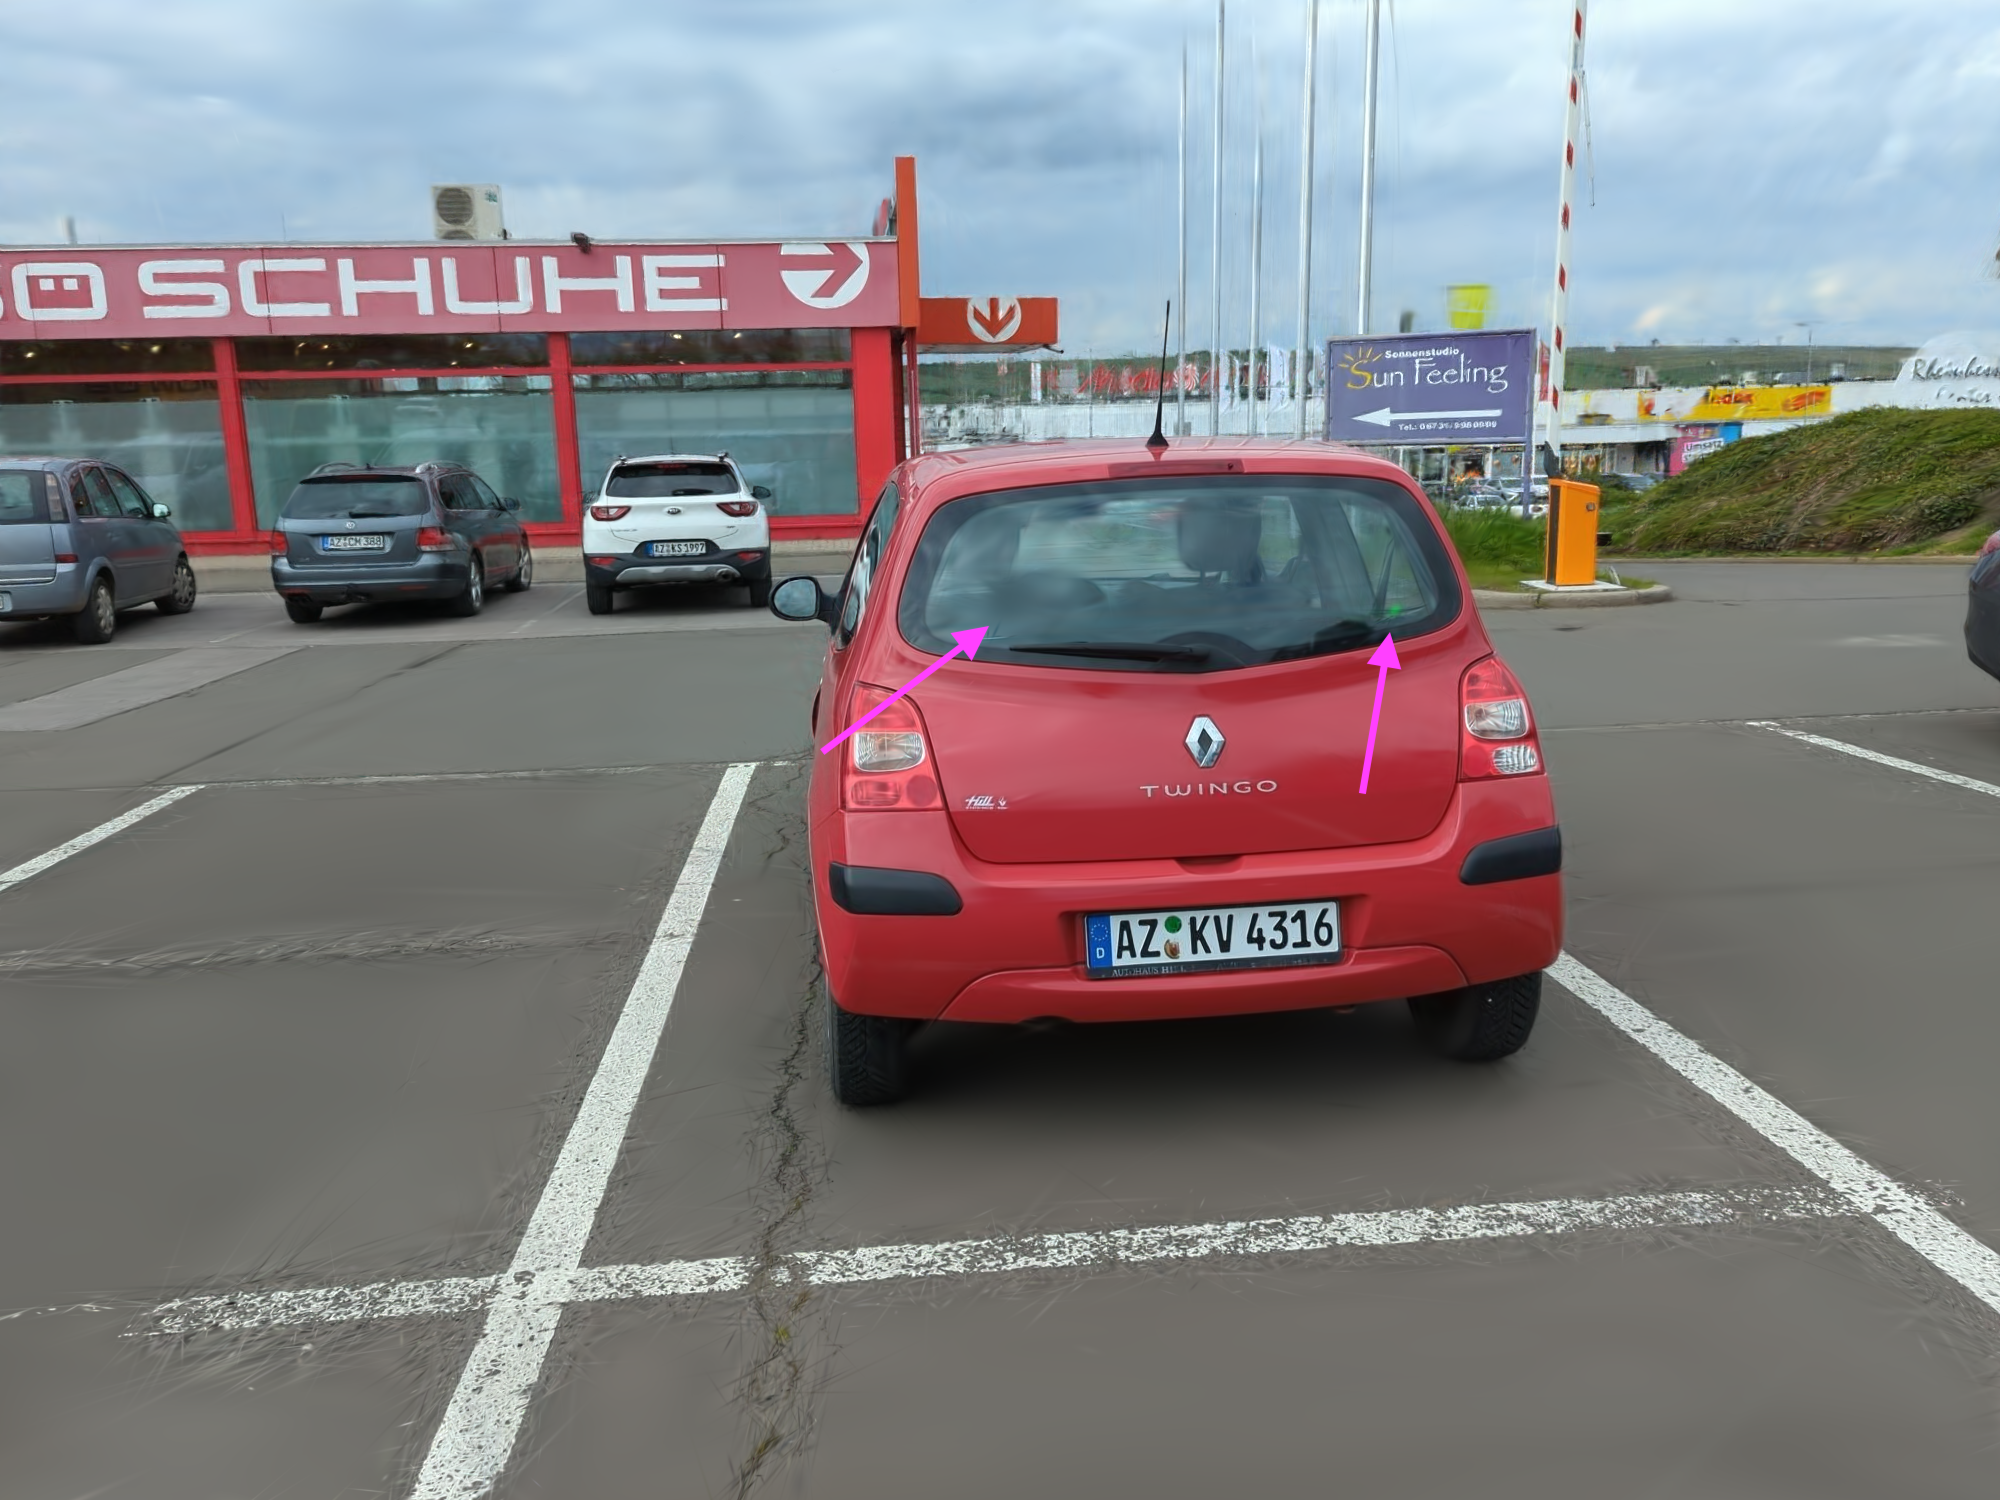
\includegraphics[width=\linewidth]{images/gaussiansplatting/00029-gs.png}
    \caption{\textbf{Vanilla GS rendered view}}
    \label{fig:view3}
  \end{subfigure}
  \quad % Space between the figures
  \begin{subfigure}[b]{0.45\linewidth}
    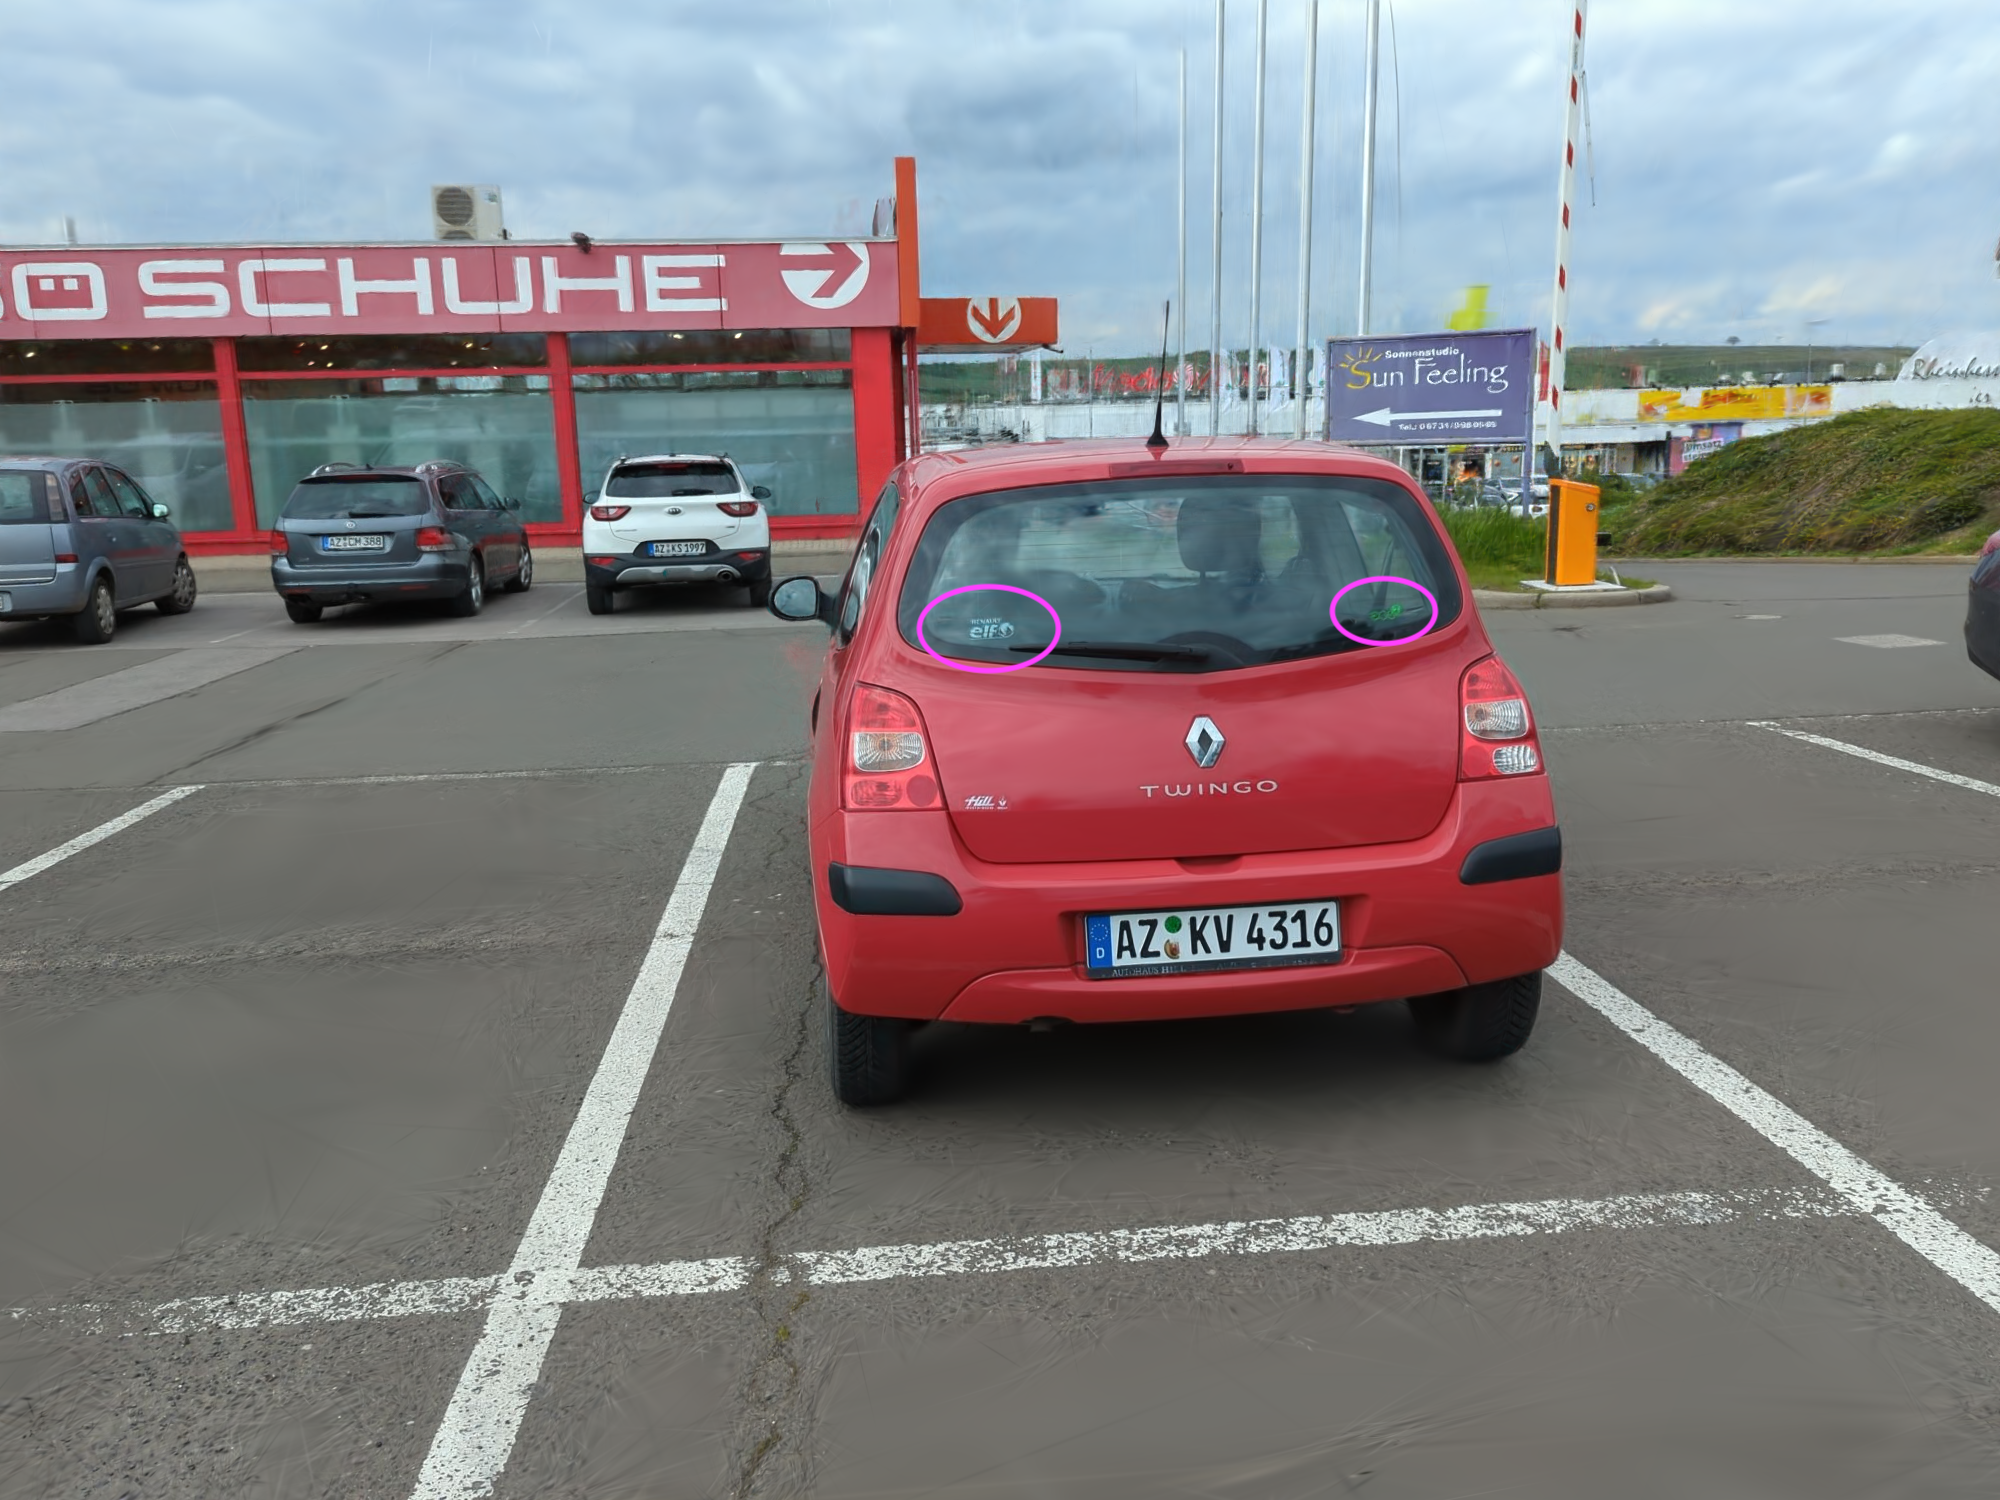
\includegraphics[width=\linewidth]{images/gaussiansplatting/00029-pixgs.png}
    \caption{\textbf{PixGS rendered view}}
    \label{fig:gs-view3-gs}
  \end{subfigure}
  \caption{\textbf{PixGS ADC influence.} Both logo on the rear windows are missing on the vanilla \ac{GS} version: nor the \textit{Renault elf} and \textit{ECO} signs are visible. PixGS, through its clever densification strategy, managed to render such complex details.}
  \label{fig:gs-pigs}
\end{figure}

Only core difference PixGS has over the vanilla 3D\ac{GS} implementation is the \ac{ADC} component. As soon as such a component is replaced in our system, rendered views immediately gain in sharpness and details: over and under-reconstructed areas are better handle by the \ac{ADC} module. Nor the viewing direction MLP or the visual hull initialisation were used in the rendered views from Figure \ref{fig:gs-pigs}. 

\subsection{Complete pipeline}

We finally conduct a complete ablation study over our different modules to emphasize on the consistency each of our modifications bring to the entire \ac{GS} pipeline system. 

Table \ref{table:gs-abaltion} summarises the impact each of our module has. Whereas both the viewing direction \ac{MLP} and the PixGS densification strategy steadily enhance all our metrics, the visual hull has only a limited impact outside the car region. Such an observation is consistent with the results presented in Table \ref{table:gs-abaltion}. 

\begin{table}[htp!]
  \caption{\textbf{Ablation study.} Influence of our different algorithm components on our $360^{\circ}$ 3D\ac{GS} system.}
  \label{table:gs-abaltion}
  \begin{adjustbox}{width=\linewidth}
  \begin{tabular}[h]{c||ccccccc}
  \hline
   Pipeline & \multicolumn{3}{c}{Full Image} & \multicolumn{3}{c}{Car only} \\
   &  SSIM ($\uparrow$) & PSNR ($\uparrow$) & LPIPS ($\downarrow$) & SSIM ($\uparrow$) & PSNR ($\uparrow$) & LPIPS ($\downarrow$)\\
  \hline
  3D\ac{GS} \citep{kerbl20233d}  & 0.798  & 28.413 & 0.325 & 0.980 & 38.668 & 0.036 \\
  + Viewing Direction & 0.808 & 29.163 & 0.318 & 0.983 & 40.917  & 0.031 \\
  + Visual Hull & 0.810 & 29.288 & 0.314 & 0.984 &41.249  & 0.030 \\
  + PixGS \ac{ADC} & \textbf{0.861} & \textbf{31.077} & \textbf{0.248} & \textbf{0.990} & \textbf{43.983} & \textbf{0.020} \\
  \hline 
  \end{tabular}
  \end{adjustbox}
  \end{table}

These metric scores are finally visually matched through the exhaustive rendered view depicted on Figure \ref{fig:gs-vh-result}. The original 3D\ac{GS} architecture fails on this rendered view to retrive tiny and complex details as the tank fuel or the car interior. Adding the viewing direction \ac{MLP} $\Phi$ before the rasterizing stage helps our training a lot. Corresponding rendered view has now a better car interior, whereas the fuel tank is still partially rendered. On top of this first modification, merging the visual hull point cloud with the one produced by COLMAP also consistently improves rendering: car exterior and interior details has been preserved and even enhanced. The tank fuel is now almost entirely rendered. Finally, the densification strategy proposed by PixGS is striking regarding tiny details. Fuel tank is perfectly rendered but the car interior is now extremely well rendered and one could struggle to distinguish the real ground truth image from the rendered one by only focusing on the car itself.   

\begin{figure*}[htb!]
  \center
\includegraphics[width=\linewidth]{images/gaussiansplatting/image_final.png}
\caption{\textbf{Cumulative influence of our different module} Each module that was implemented in our system consistently bring its own contribution without deteriorating what was improved by former bloc. Car interior and fuel tank details are progressively improved until our final system model.}
\label{fig:gs-vh-result}
\end{figure*}

\section{Limitations}
\label{sec:gs-limitation}

Wheareas our 3D reconstruction pipeline is able to faithfully render and synthesize novel view at training (\textit{in-distribution}) locations, moving too far war away from the original camera path might lead to severe artefact at render time. One of the most known undesired effect for 3D\ac{GS} scene is often termed \textit{floater} artifacts. We illustrate on Figures \ref{fig:floater-limitation} and \ref{fig:floater-removed} this effect\footnote{We illustrate this limitation on another scene since the one we used in this chapter is not prone to floater artifacts.} and how it can easely be handled by narrowing the viewing camera frustrum at inference time. These artifacts are rendered when $z_{min}=0.2$ since associated gaussians primitives has the required minimal depth to be rendered during the rasterization stage. Increasing the minimal depth to $z_{min}=1.2$, any primitive that does not meet this depth requirement will not be rendered, as it no longer falls within the newly narrowed camera frustum.

\begin{figure*}[htb!]
  \center
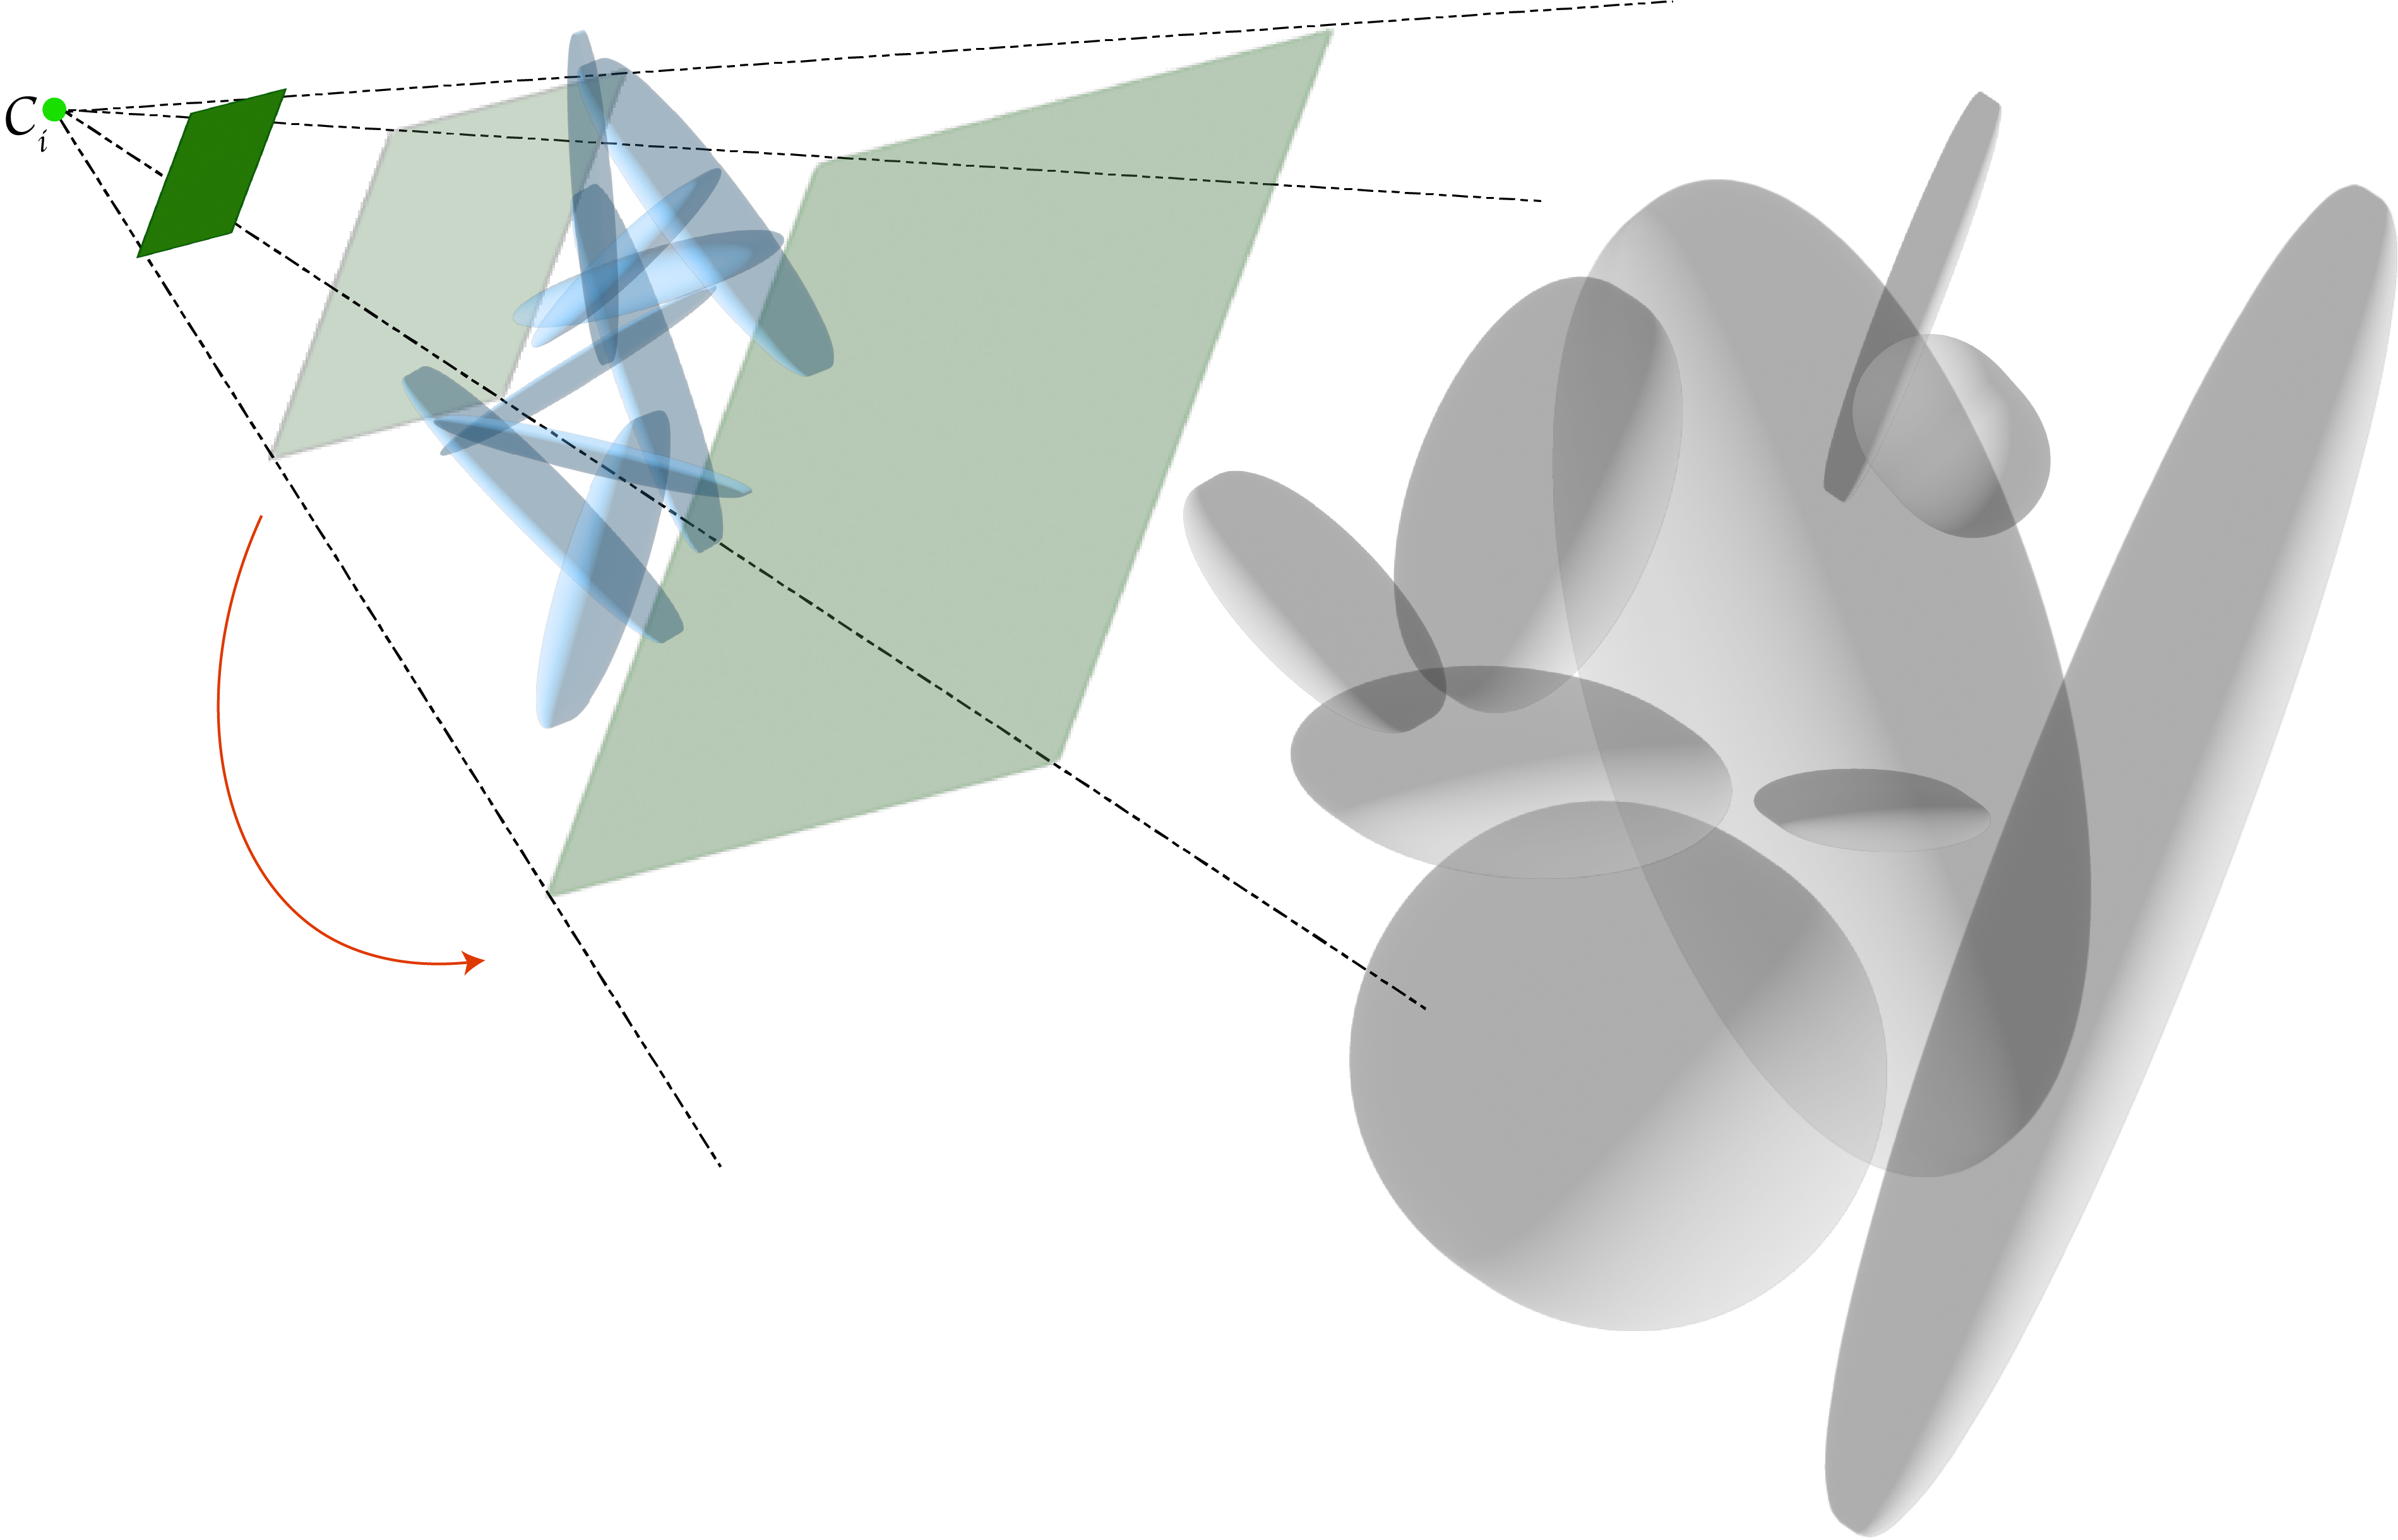
\includegraphics[width=.7\linewidth]{images/gaussiansplatting/gaussian-floaters.png}
\caption{\textbf{Toy illustration for camera frustrum narrowing.} Increasing the minimal depth at which gaussian primitives are rasterized or not allows to avoid undesired gaussians being rendered at non-training locations.}
\label{fig:floater-limitation}
\end{figure*}

\begin{figure}[htb!]
  \centering
  \begin{subfigure}[b]{0.45\linewidth}
    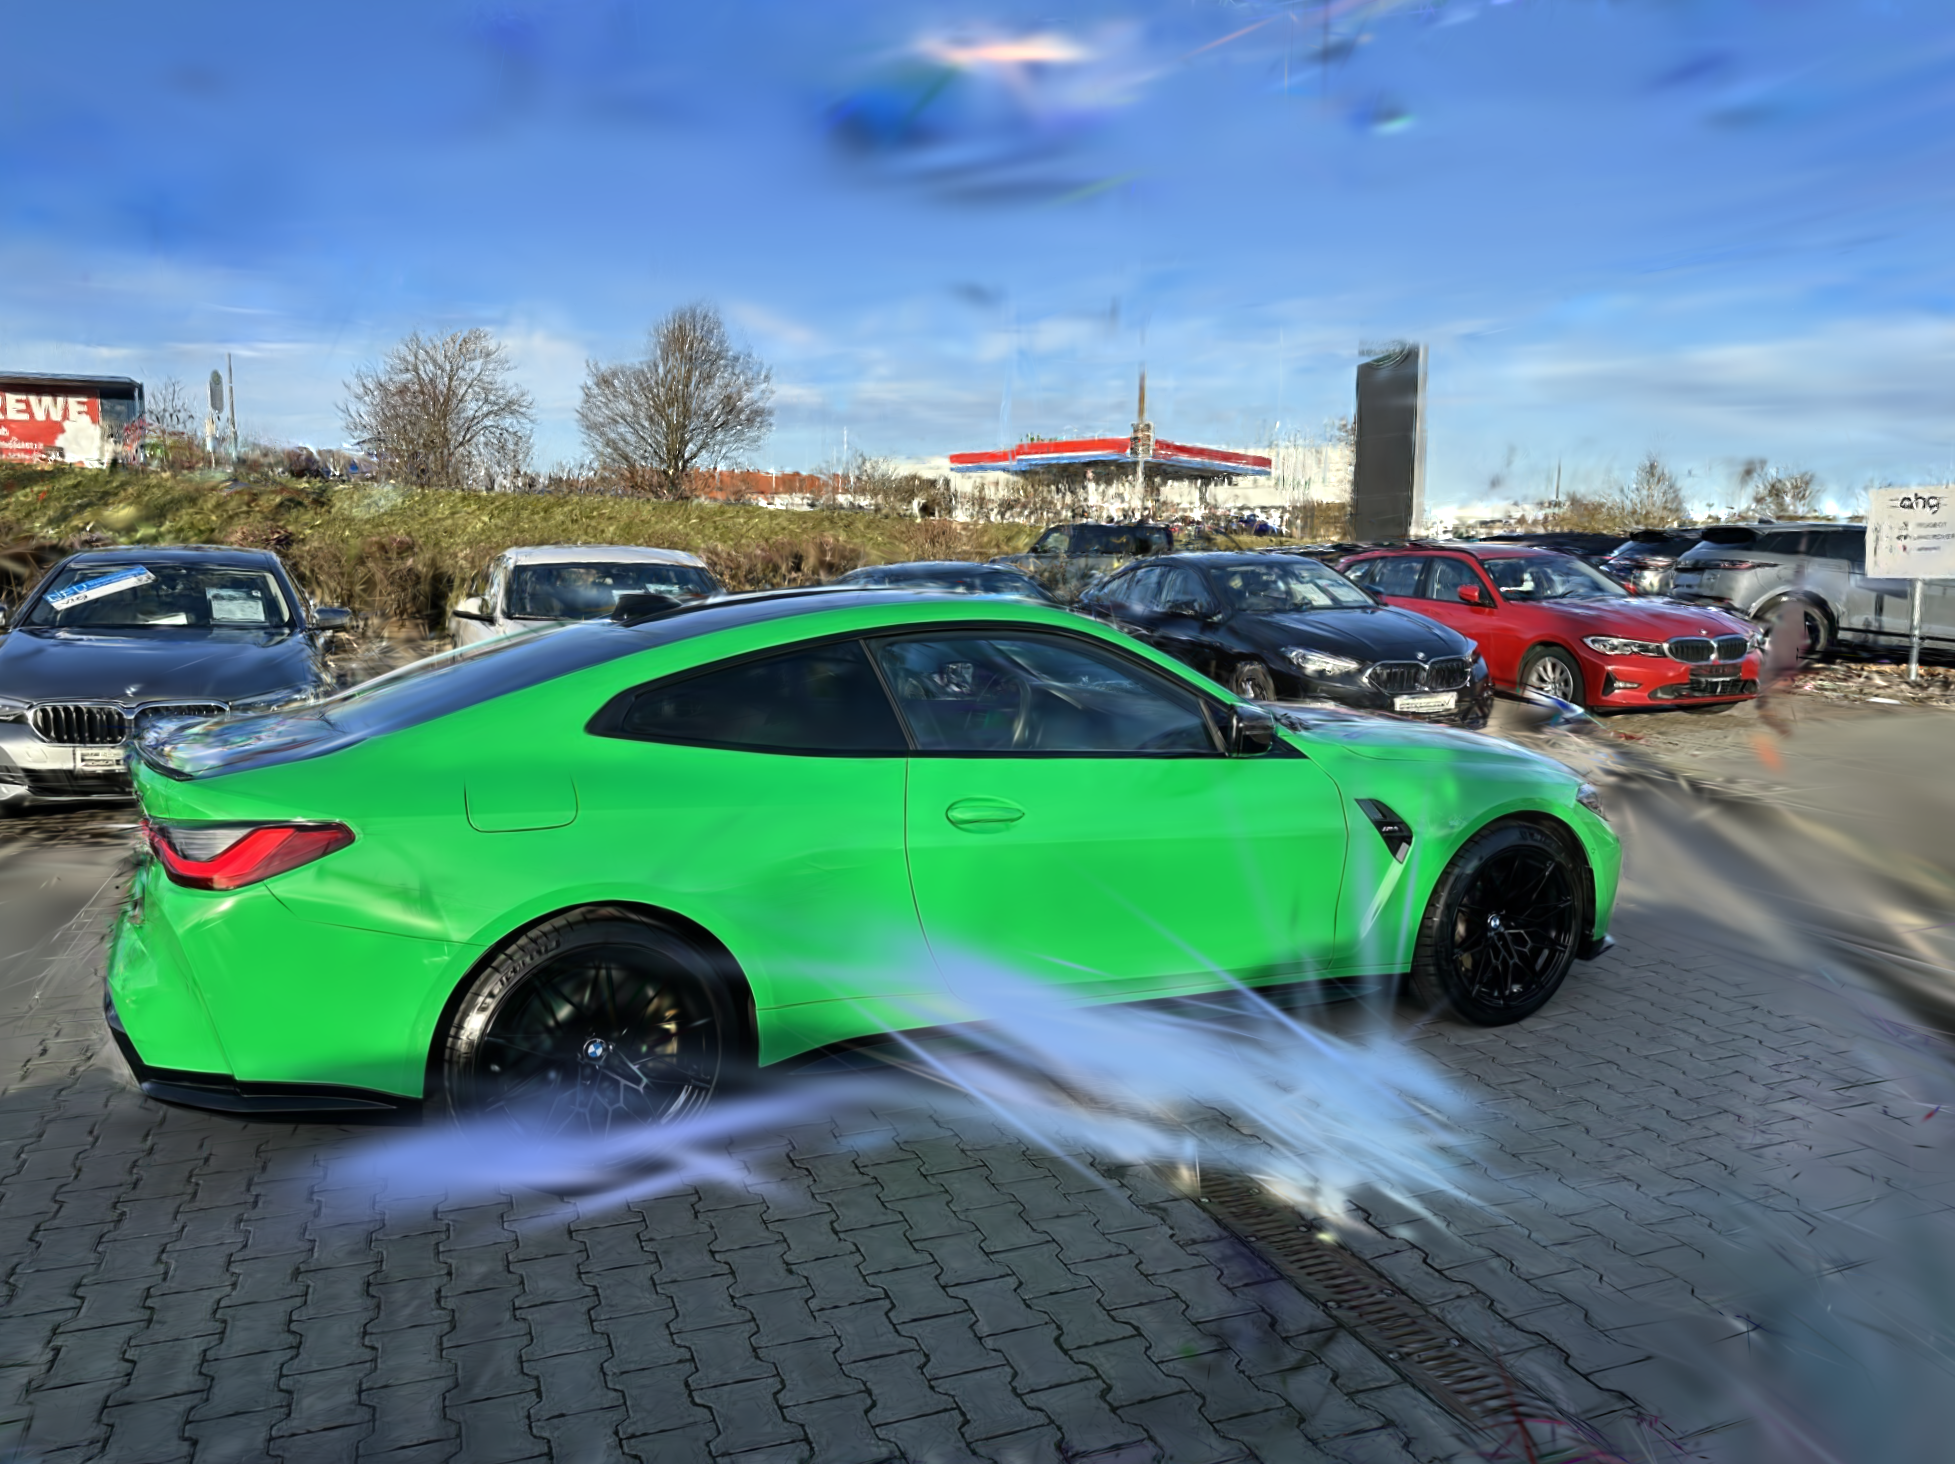
\includegraphics[width=\linewidth]{images/gaussiansplatting/needle-artifact.png}
    \caption{\textbf{Rendering with $z_{min}$=0.2} }
  \end{subfigure}
  \quad % Space between the figures
  \begin{subfigure}[b]{0.45\linewidth}
    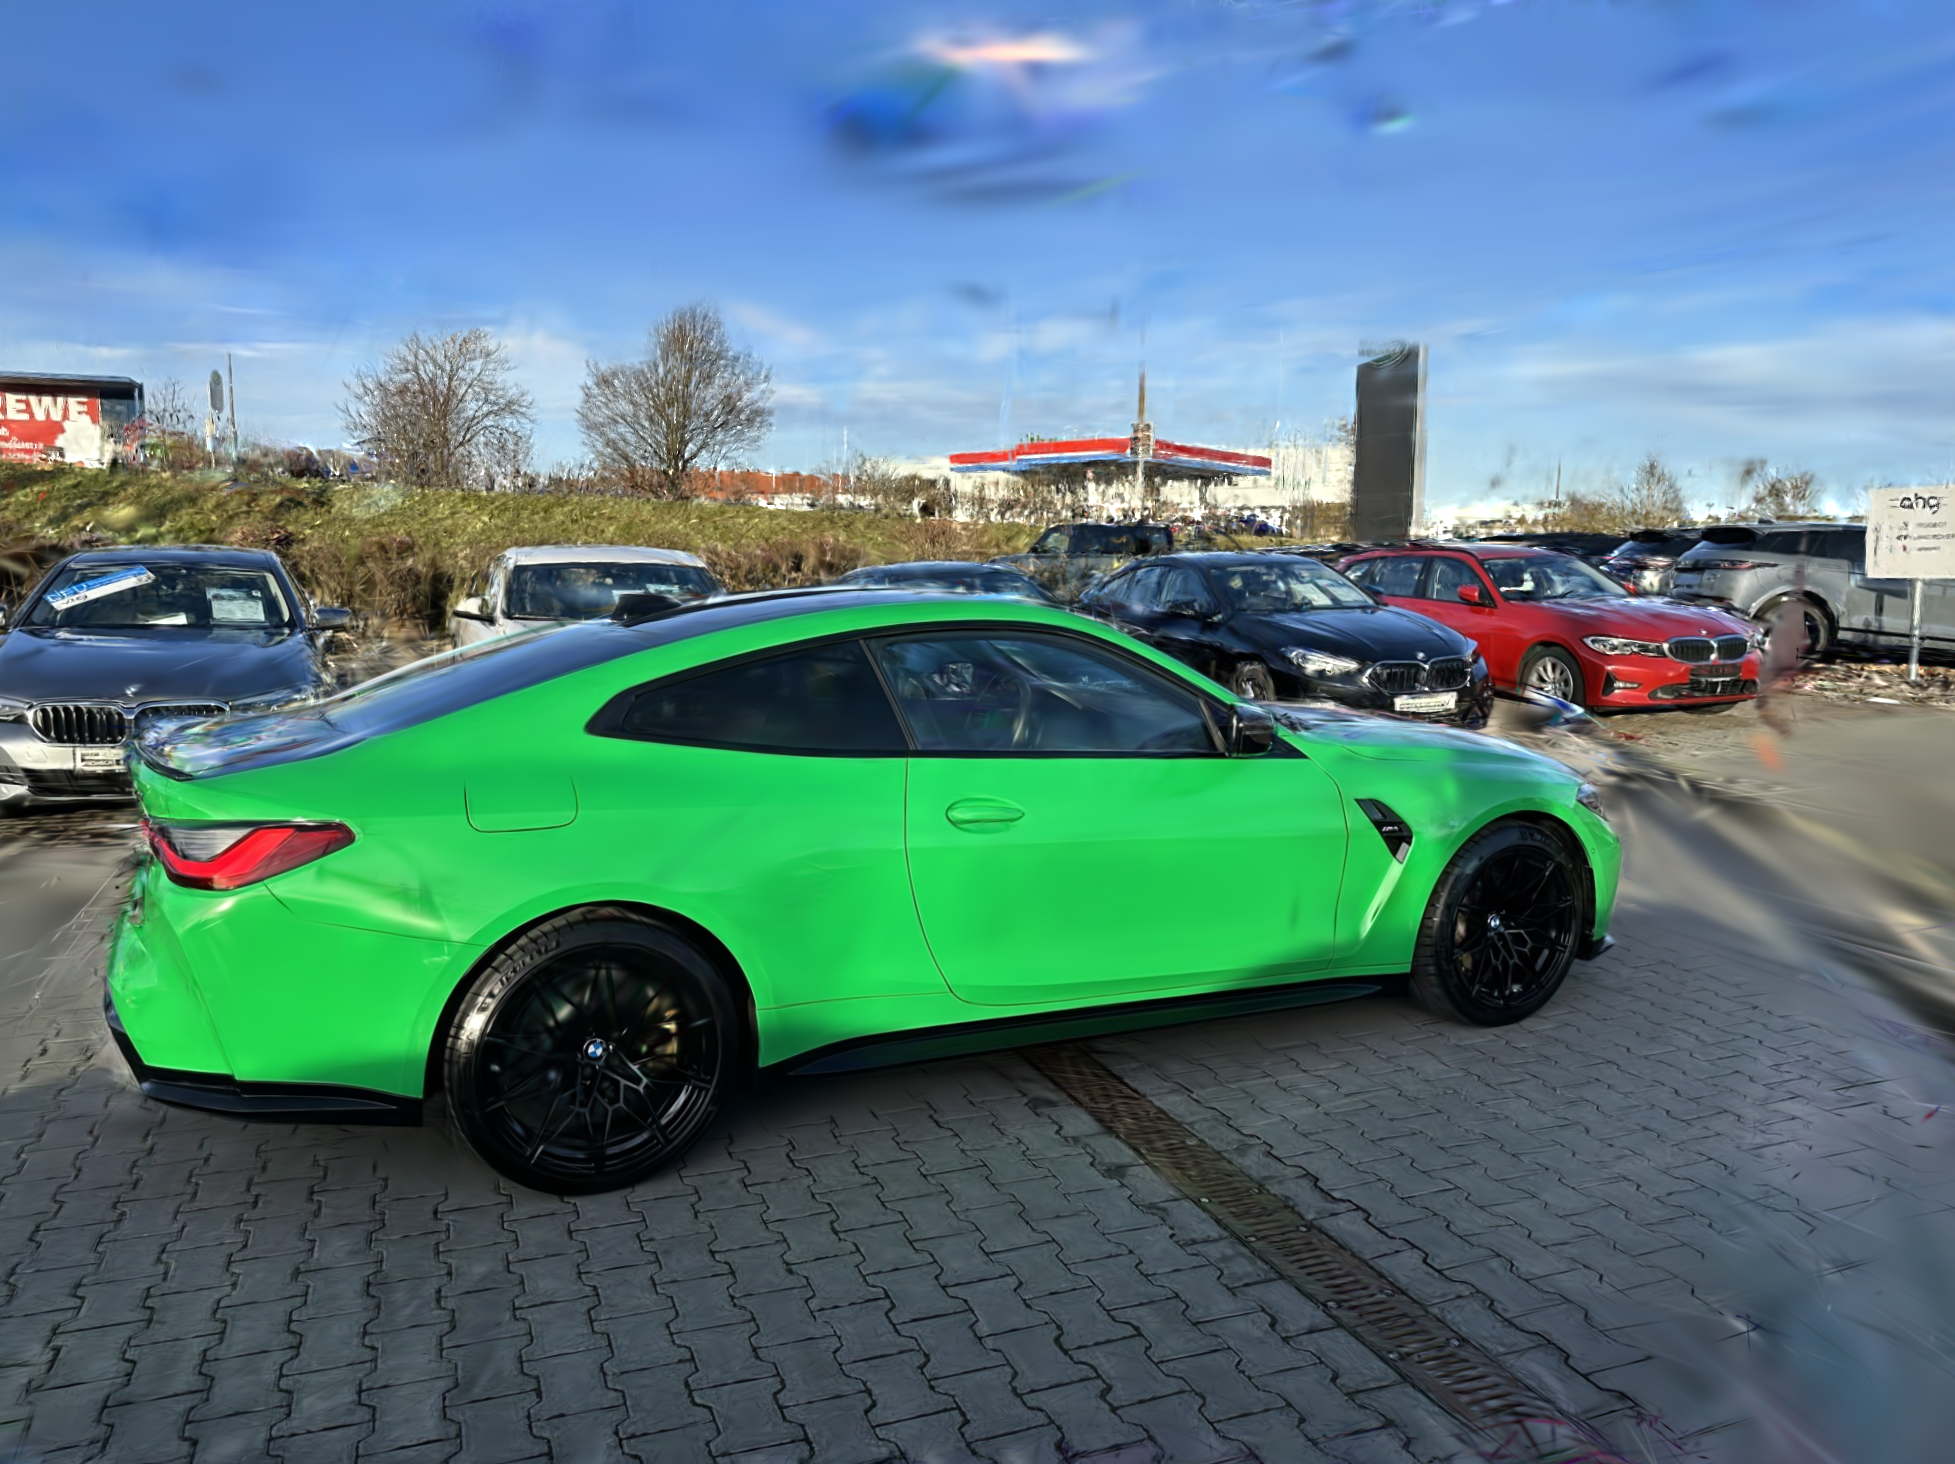
\includegraphics[width=\linewidth]{images/gaussiansplatting/needle-free-artifact.png}
    \caption{\textbf{Rendering $z_{min}$=1.2} }
  \end{subfigure}
  \caption{\textbf{Camera frustrum impact on floater artifacts.} Slightly changing the minimal depth value at which gaussian primitives are rendered or not on the image plane has a huge impact on the final image. Increasing such minimal depth value allows to get ride of those floater primitives.}
  \label{fig:floater-removed}
\end{figure}

Beyond the rendering of these unwanted gaussian primitives, rendering at non-training locations remains a challenging tak that would need to be handled in further research. Indeed, only having a sparse set of 36 views to reconstruct a whole scene remains complex: public datasets on which 3D\ac{GS} is trained on for academic purposes often have a few hundreds of images. In our case, views have to be rendered at locations that are slighly different the original training ones, as depicted on Figure \ref{fig:theory-camera-path}. 

\begin{figure*}[htb!]
  \center
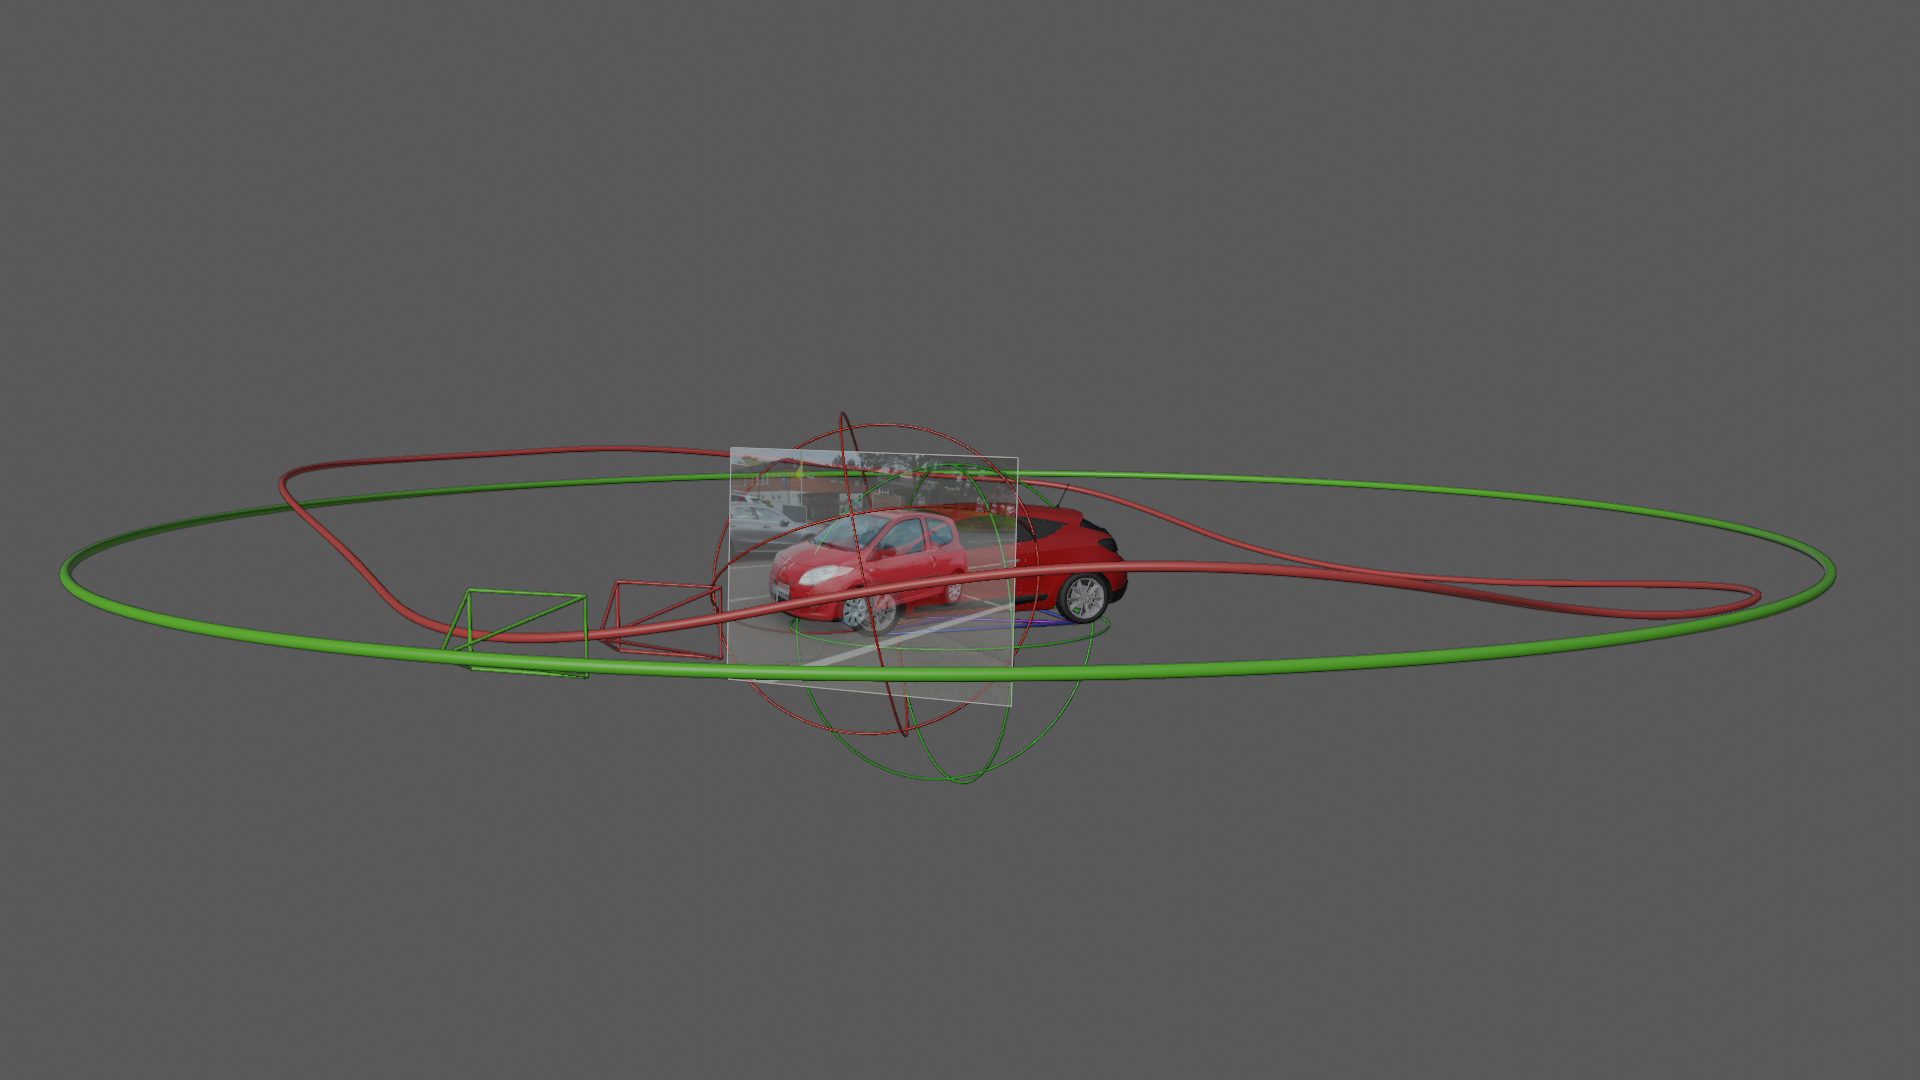
\includegraphics[width=\linewidth]{images/gaussiansplatting/theory-camera-path.png}
\caption{\textbf{Camera path stabilization.} While the original camera path associated to the input views is plotted in red, the $360^{\circ}$ spin stabilization require rendering of our learned 3D scene at camera locations that live on the green path.}
\label{fig:theory-camera-path}
\end{figure*}

The figure \ref{fig:nontraining-rendering} in practice illustrates this common case we faced when we need to stabilize a scene. The 3D\ac{GS} scene is extremely well rendered at this training location, even though the ground surface and the sky suffer from a lack of gaussian primitives in those over-reconstructed regions. Moving closer to the car, at a non-training location, lead to a rendering that is far from being acceptable for an industrial application. Several artifacts and misplaced or misoriented gaussians appeared on the back of the car, leading to a blurry and fuzzy result. 

\begin{figure}[htb!]
  \centering
  \begin{subfigure}[b]{0.45\linewidth}
    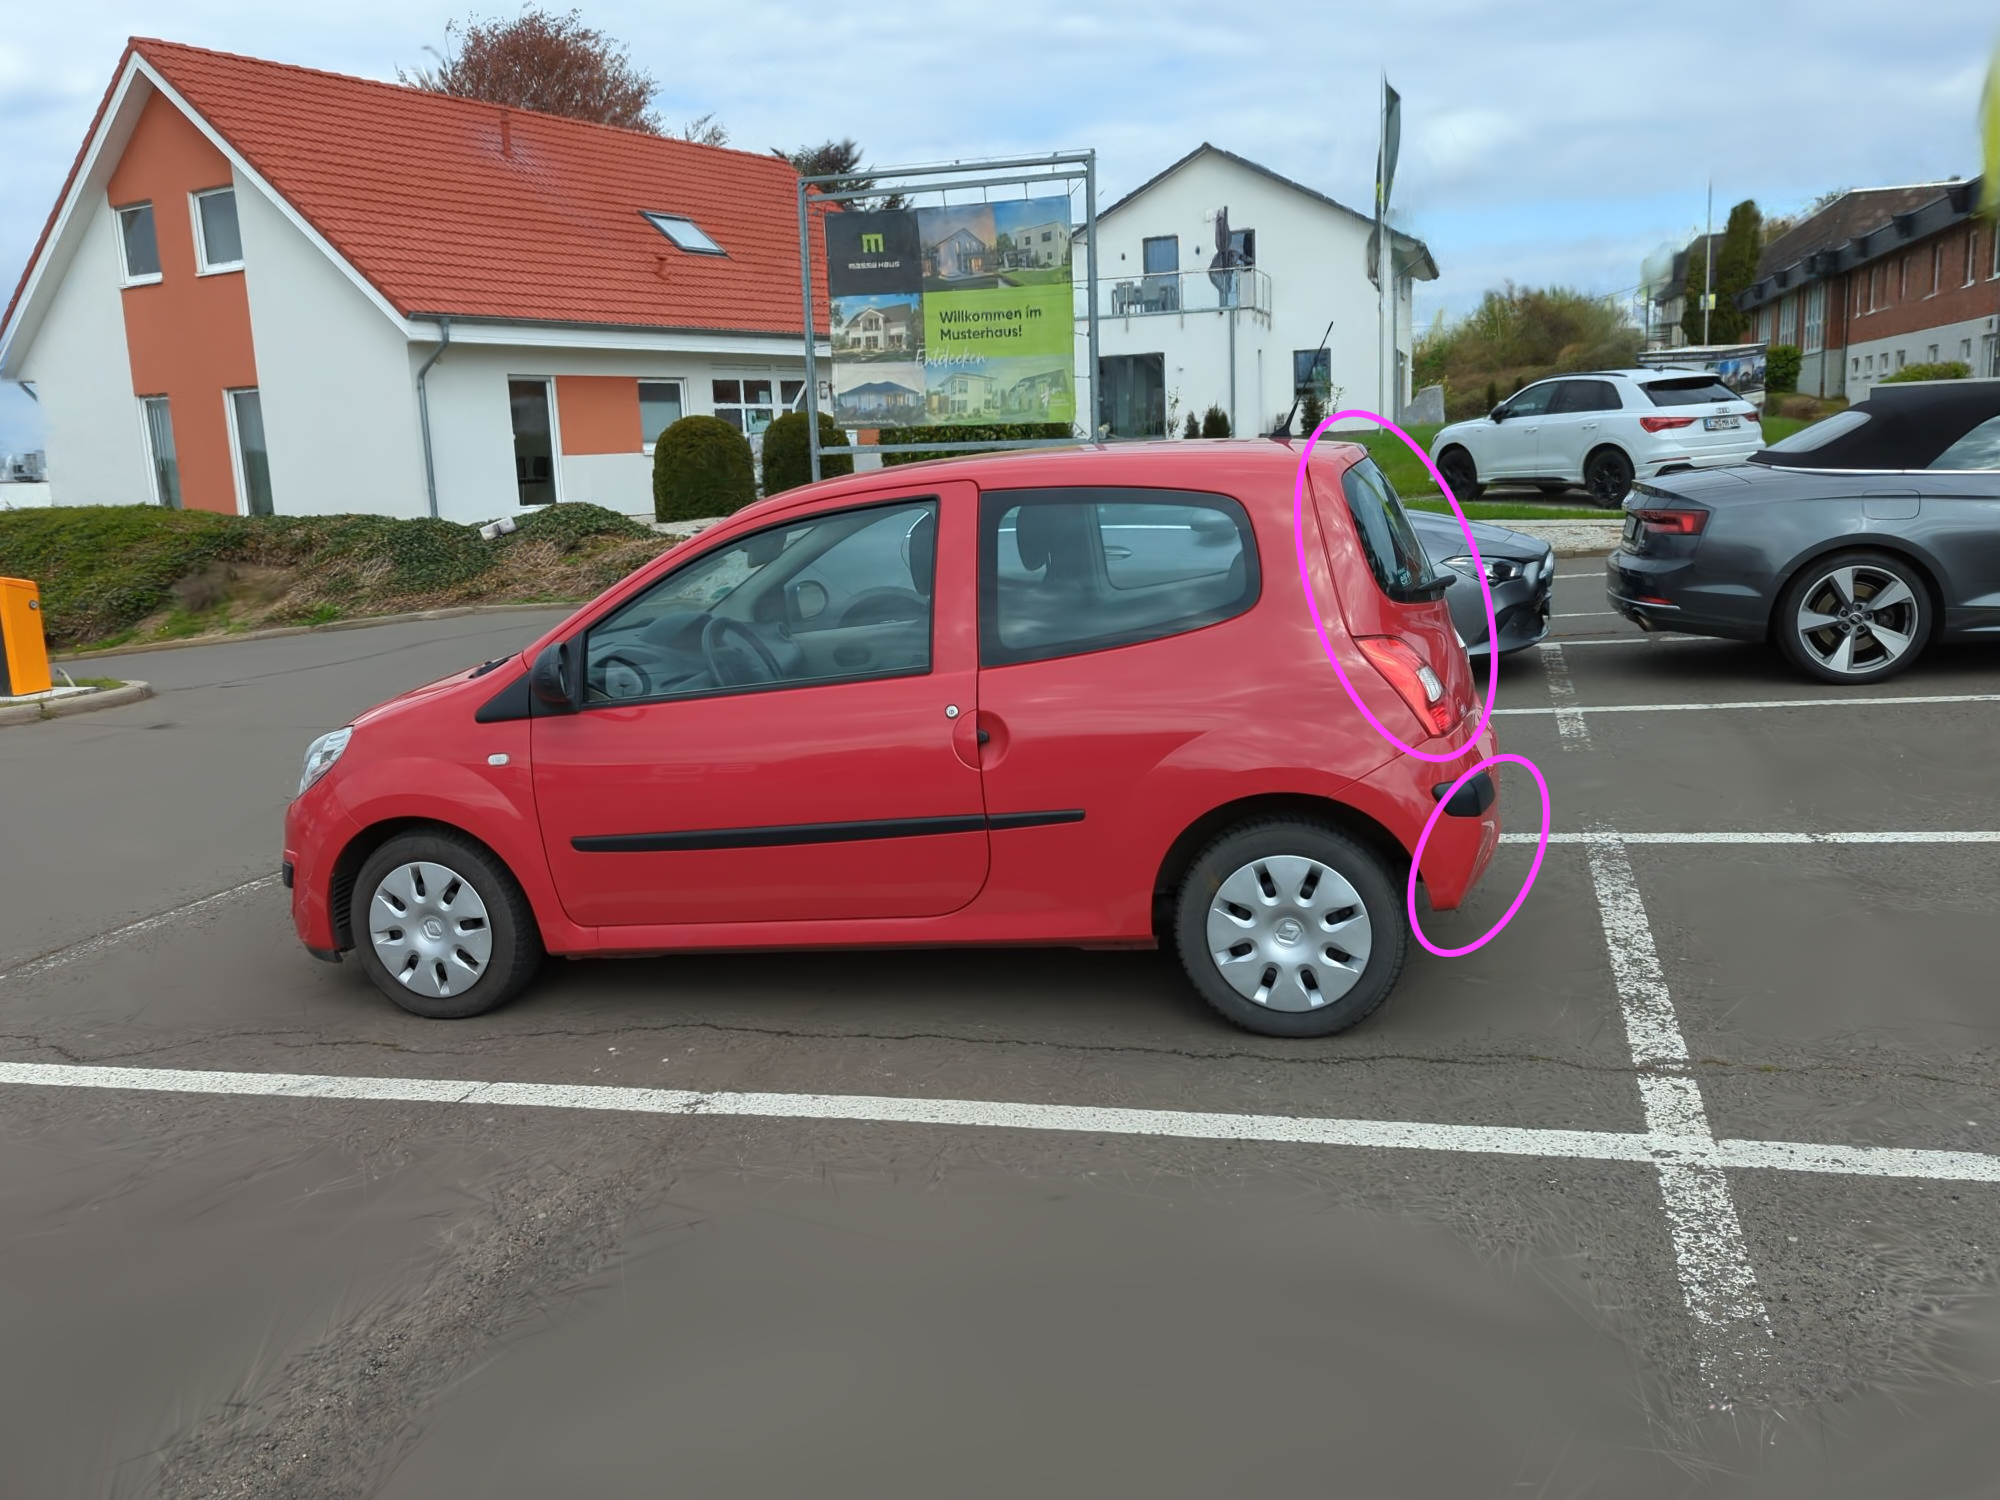
\includegraphics[width=\linewidth]{images/gaussiansplatting/00023-unstabilized.png}
    \caption{\textbf{Rendering at training location (unstabilized).}}
  \end{subfigure}
  \quad % Space between the figures
  \begin{subfigure}[b]{0.45\linewidth}
    \includegraphics[width=\linewidth]{images/gaussiansplatting/00023-stabilized.png}
    \caption{\textbf{Rendering at non-training location (stabilized).}}
  \end{subfigure}
  \caption{\textbf{Main limitation for $360^{\circ}$ spin stabilization.} While a rendering at a training location gives appealing result, moving ahead and tring to render the same scene at this new location remains a challenging case that is currently unproperly adressed.}
  \label{fig:nontraining-rendering}
\end{figure}

\section{Current research line of work}

Whereas improving the 3D rendering at non-training locations remains one of the core challenges ahead for further research, current work is mostly focused toward geometrical priors integration within the 3D\ac{GS} pipeline that was described earlier. 

Indeed, introducing depths and normals regularization during training enforce gaussian primitives to better model the car surface in 3D. 
We thus currently leverage on a monocular depth \citep{ke2023repurposing,yang2024depth} and normal \citep{bae2024rethinking,ye2024stablenormal} estimation networks to obtain these \textit{pseudo} ground truth depths and normals maps and use them as prior information during training. 

The discrete volume rendering approximation from Equation \eqref{eq:gs-alpha-blending} is adjusted to render per-pixel z-depth estimates $\hat{D}$:

\begin{equation}
  \hat{D}(x) = \sum_{k=1}^{K} d_{k}\alpha_{k}\prod_{j=1}^{k-1}(1-\alpha_{j})
\end{equation}
with $d_{k}$ the z-depth coordinate (in view space) of the $k^{th}$ primitive. \newline

Gaussian's normal might be set as an additional learnable attribute. However, we rather decided to define the normal $n_{k}$ of a gaussian primitive $\mathcal{G}_{k}$ as the outward direction given by its shortest axis. In this way, $n_{k}$ can directly be expressed (in the world coordinate system) from the scaling $s_{k}$ and quaternion $q_{k}$: 

\begin{equation}
  n_{k} = R_{k}\mathbf{e}_{\arg\min_{j}(s_k)}
\end{equation}

where $R_{k}$ correspond to the $3\times 3$ rotation matrix associated to quaternion $q_{k}$ and $e_{l}$ defines the standard basis vector (the one-hot vector) with $1$ in the \textit{l}-position and $0$ elsewhere.  

Such formulation allow us to slighlty adapt the input of the \ac{VDGS} network, to only input normals and the viewing direction. 

\section{Conclusion}

We develop in this last chapter a 3D reconstruction pipeline to perform \ac{NVS} for an industrial application. We leverage onto original 3D\ac{GS} \citep{kerbl20233d} work to design a system that suits the specific requirements Meero has regarding $360^{\circ}$ spin stabilization. In this way, we extend the original 3D\ac{GS} architecture with three main components: a visual hull point cloud initialization, a view-dependent opacity correction and a better densification strategy. Each of these modules directly tackle an issue that original 3D\ac{GS} was not able to deal with. First, the visual hull point cloud enables to start the training process with more points on the surface of interest, \ie the car we aim to reconstruct. Then, gaussian primitives opacity are made view-dependant through a \ac{MLP}. Such a network allows to better render reflective and transparent surfaces, such as windows. Finally, the \ac{ADC} strategy proposed by PixGS \citep{zhang2024pixel} has a significant positive impact to render intricate details and complex structures. Furthermore, such a novel \ac{ADC} strategy does not hurt training time as only a pixel area scaling term need to be computed. We extensively test our entire pipeline onto a single scene, that could have been one of a Meero client, through different ablation studies. One of the core limitation remain the rendering at non-training locations, \ie at stabilized positions in our case. Several artifacts can appear when the 3D scene is rendered at those unseen and out-of-distribution camera positions. Further works around geometrical priors will try to adress this main limitation in a near future. 
